\section{Introduction}
\label{sec:generalisation_intro}
Recent years have seen significant advancements in the use of deep learning for the dermatological classification of skin lesion images~\citep{du2020ai,wu2022skin}. Deep learning classifiers have been shown to be particularly effective with large datasets, such as the ISIC archive, which have enabled substantial progress in this field~\citep{tschandl2018ham10000,wen2021characteristics}. Studies utilising high-quality datasets have reported performance that is comparable to or surpasses that of dermatologists in the classification of skin lesions~\citep{esteva2017dermatologist,haenssle2018man,han2018classification,tschandl2019expert}. Additionally, research has investigated the ability of deep learning classifiers to accurately classify macroscopic clinical images, as opposed to solely dermoscopic images~\citep{fujisawa2019deep}. However, it should be noted that images acquired from primary care settings are often of variable quality, with wider and less consistent fields of view or focus, and may include visual distractions.

Current deep learning classifiers for medical images have been observed to exhibit poor generalisation across different healthcare systems, acquisition protocols, and patient populations. This phenomenon has been documented in several studies, with evaluations typically being conducted in an internal manner, where the model training and testing datasets are drawn from the same source (e.g., \cite{han2018classification}). However, there remains a significant degree of uncertainty regarding the ability of these models to generalise across diverse domains, datasets, and imaging modalities. 

Given the complexity of the medical imaging domain, it may be unrealistic to expect the development of a universally applicable skin lesion classifier. A more practical approach may involve the utilisation of local datasets to adapt models to specific target populations and healthcare systems. This approach would involve leveraging the knowledge acquired from these datasets to fine-tune existing models, thus increasing their applicability and performance within specific domains. This approach has been proposed in several studies and is considered a more realistic and practical solution to the challenges of generalisation in deep learning-based medical image analysis~\citep{glocker2022risk}. 

The phenomenon of domain shift, wherein the distribution of features in the new population diverges from the distribution of features present in the training data, has been identified as a major obstacle in the deployment of artificial intelligence systems in clinical environments. This issue has been identified as a crucial challenge in implementing artificial intelligence systems in clinical settings, as highlighted in \cite{kelly2019key}. Additionally, this weakness arising from domain shift can result in unintended consequences such as gender or racial discrimination bias~\citep{glocker2022risk}. The utilisation of medical datasets for the training of deep learning models is often hindered by the lack of diversity, which is often derived from a single source with a specific population distribution. Domain shift can also occur due to differences in the image capture methods, such as differences in the intensity distribution of MRI scanners at different sites~\citep{prados2017spinal} or staining of histological slides~\citep{stacke2020measuring}. These complexities pose significant challenges in delivering artificial intelligence systems in clinical settings.

The creation and curation of labelled datasets can be a costly and time-consuming task, as highlighted in recent studies such as \cite{chin2022prepare}. To address this issue, transfer learning~\citep{weiss2016survey} has emerged as a valuable approach for utilising knowledge acquired from large datasets in other domains and applying it to a target domain with limited data. This method has been widely adopted in the field of medical image analysis, as it allows for the fine-tuning of features learned from large datasets for use in smaller datasets within the medical domain. The effectiveness of transfer learning, however, is dependent on the similarity between the source and target domains, as well as the deep learning models utilised, as noted in studies such as \cite{matsoukas2022makes}. For instance, the utilisation of knowledge acquired from the large ImageNet dataset~\citep{deng2009imagenet} has been extensively applied in medical image analysis, despite the visual dissimilarity between the images in ImageNet and medical images. This approach has been demonstrated to be effective in the deep classification of the ISIC 2019 dermoscopy dataset, with evidence of feature re-use~\citep{matsoukas2022makes}.

In this chapter, the effectiveness of transfer learning between dermatology datasets is investigated with a focus on the utilisation of deep learning models to assist in the diagnosis of skin lesions based on community images acquired with limited control. The effectiveness of transfer learning is expected to be dependent on the size of the source datasets used for pre-training, as well as the similarity between these source datasets and the target datasets.

To explore this topic, two types of deep learning models with different inductive biases are focused on. The performance of these models is evaluated in relation to two novel datasets, specifically designed to simulate a real-world clinical setting. These datasets were gathered, trained, and tested in the context of image referrals sent to secondary-care hospital-based dermatologists from primary care. This use case was selected as it represents a common scenario in dermatology in the UK and aims to reliably identify common benign conditions in this setting.

The results from the experiments with fine-tuning between the different dataset shows that’s performance is based on the proximity of the training distribution to the testing distribution. Therefore, it is critical to obtain data from the specific real-world setting in which the deep learning will be deployed. By training, and testing on two datasets, one from primary care and the other from referred images sent for medical photography, aims to demonstrate that the approach is effective in a real-world clinical setting and can be used for triage experiments.

The work discussed in this chapter is yet to be published but is intended for submission to the British Journal of Dermatology, under the authorship of Jacob Carse, Gillian Chin, Charlotte Proby, Emanuele Trucco, Colin Fleming, and Stephen McKenna. The personal contribution to this collaborative effort is reflected in the experiments carried out on the fine-tuning of the dataset.



\section{Datasets}
\label{sec:generalisation_datasets}
In this chapter, two datasets of community-acquired macroscopic (non-dermoscopic) images were curated. These datasets were extracted from previously stored images referred from primary to secondary care in Tayside and Forth Valley, United Kingdom. The inclusion of these datasets allows for the examination of a diverse range of macroscopic images acquired in a community setting. Both sets of images were annotated using the same procedure, explained in Section~\ref{subsec:annotation_procedure}.

\begin{figure}
	\centering
	\captionsetup[subfigure]{singlelinecheck=false}
	\begin{tabular}{ccc}
		\subcaptionbox{\centering Tayside Melanoma}{\includegraphics[width=0.3\textwidth]{images/TAY_MEL.jpg}} &
		\subcaptionbox{\centering Tayside Melanocytic Nevus}{\includegraphics[width=0.3\textwidth]{images/TAY_NV.jpg}} &
		\subcaptionbox{\centering Tayside Benign Actinic Keratosis}{\includegraphics[width=0.3\textwidth]{images/TAY_BKL.jpg}} \\
		\subcaptionbox{\centering Forth Valley Melanoma}{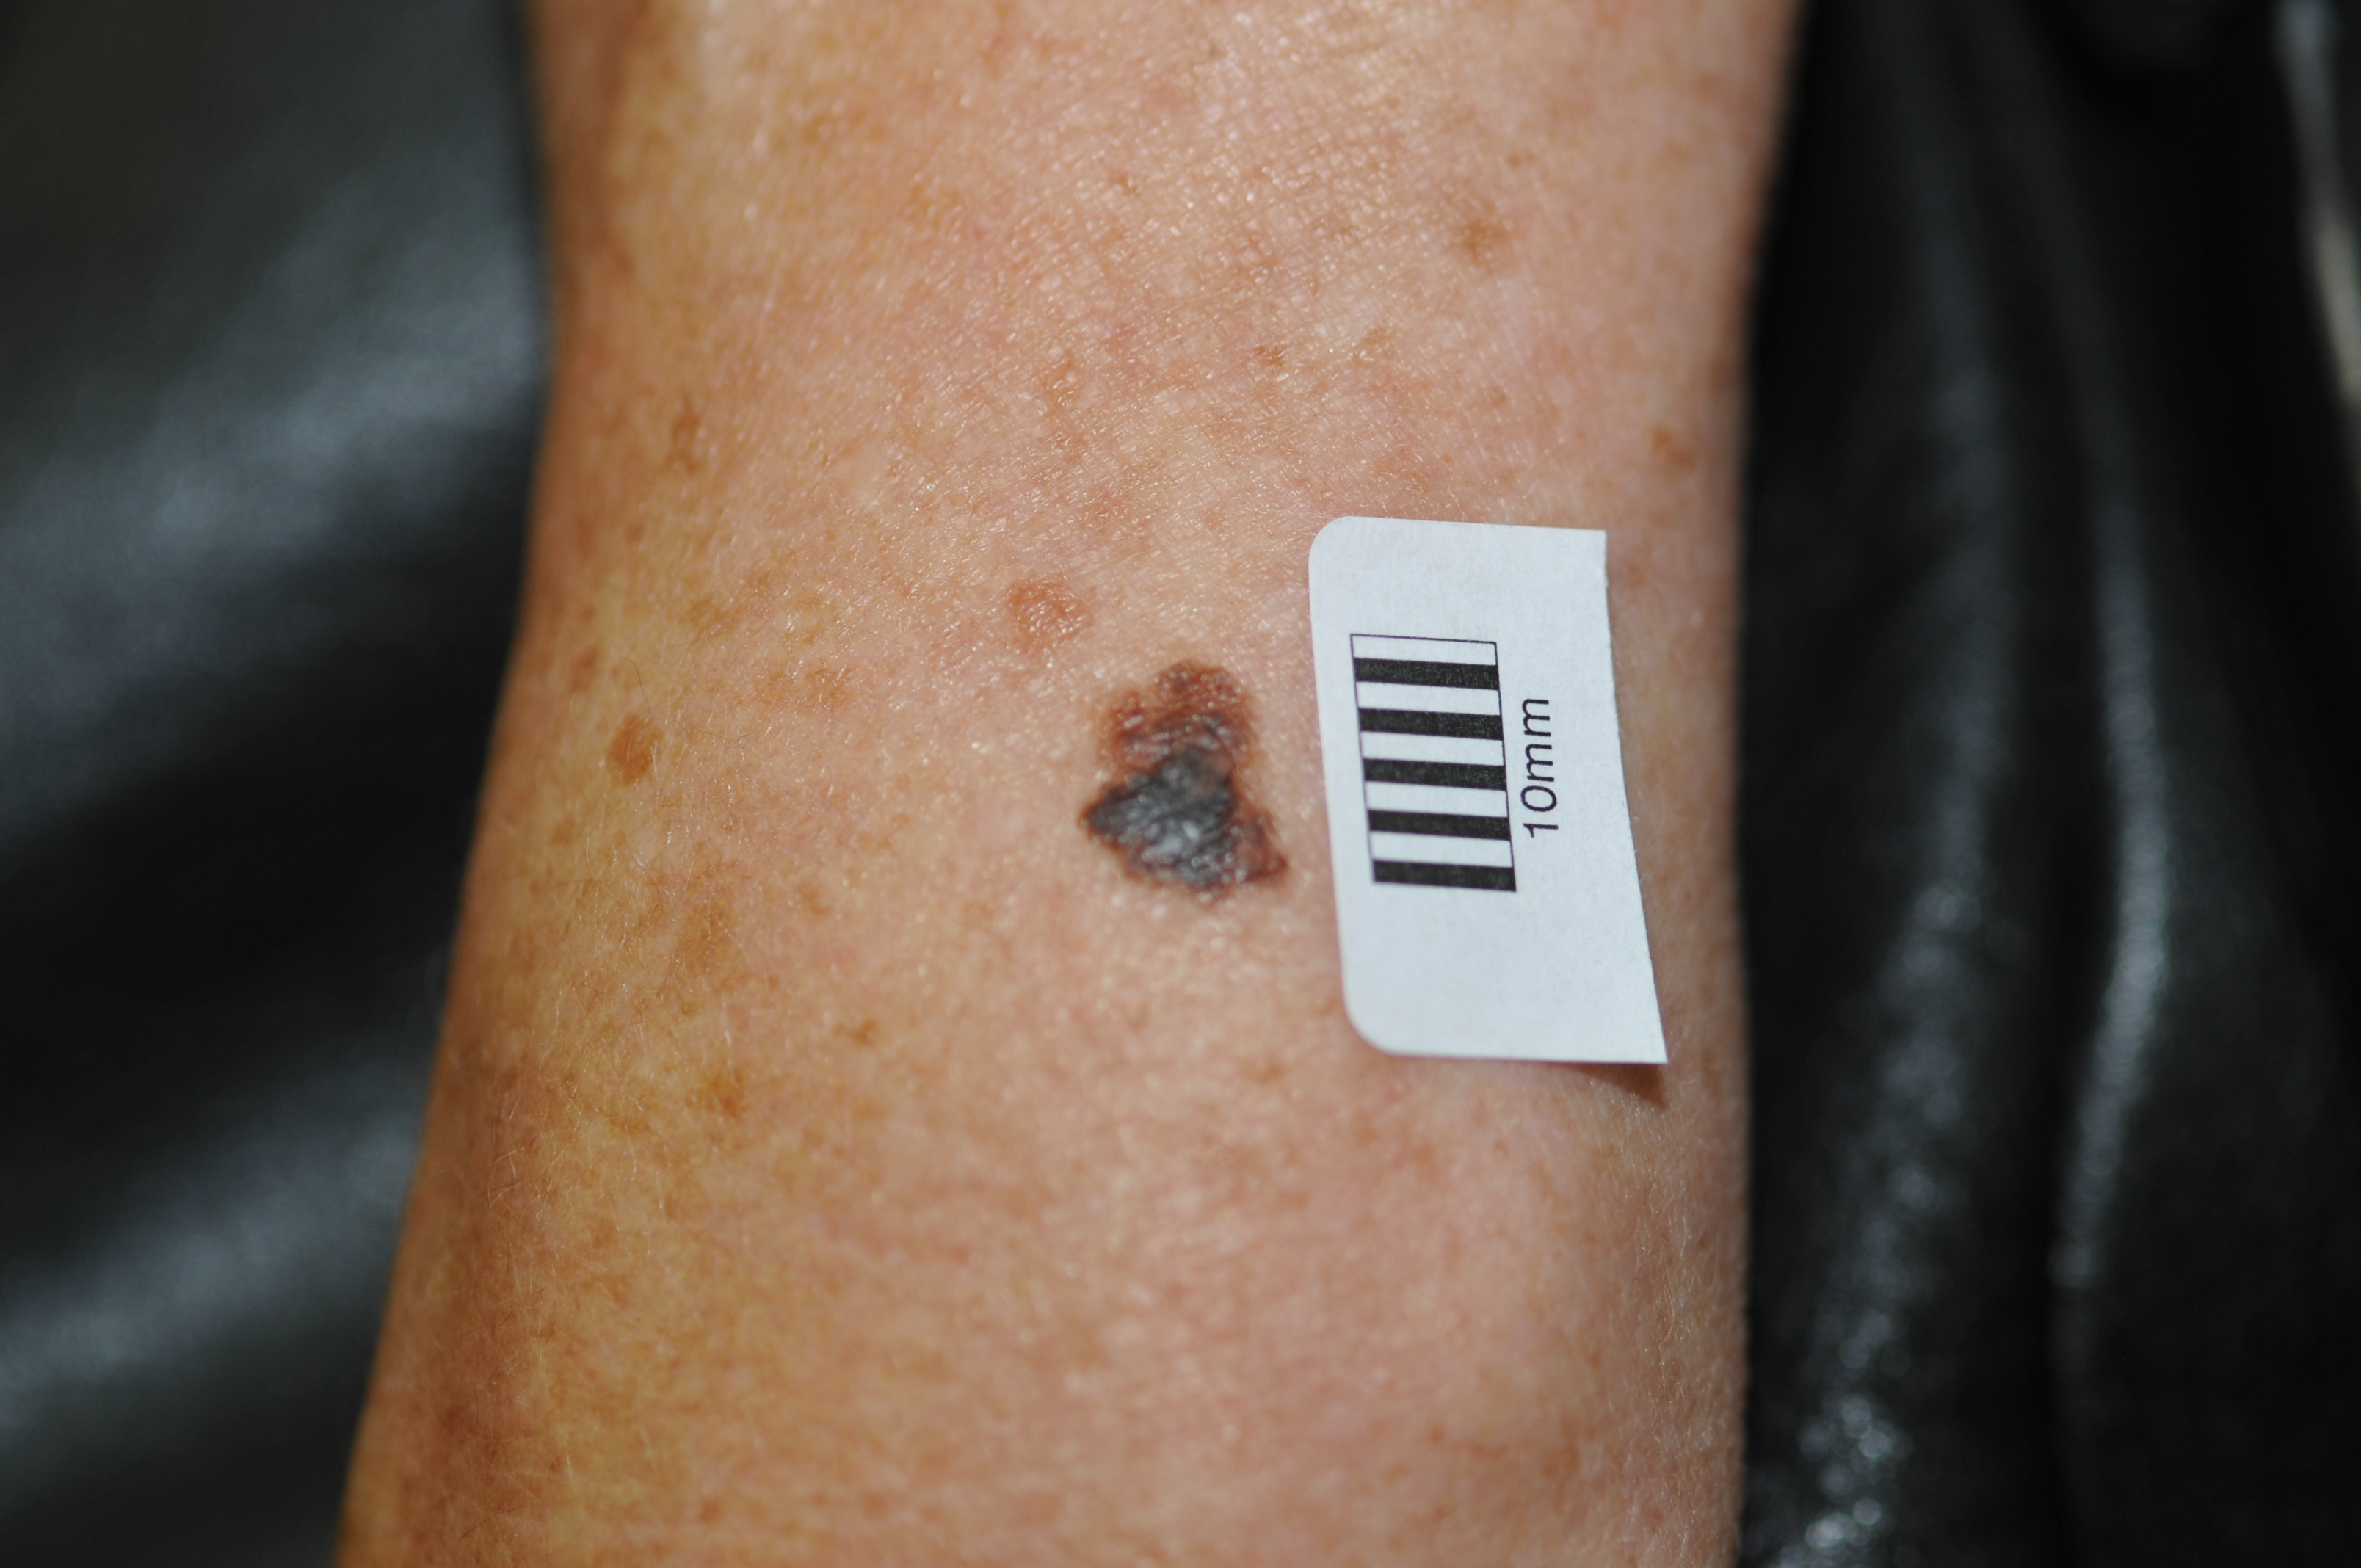
\includegraphics[width=0.3\textwidth]{images/FV_MEL.jpg}} &
		\subcaptionbox{\centering Forth Valley Melanocytic Nevus}{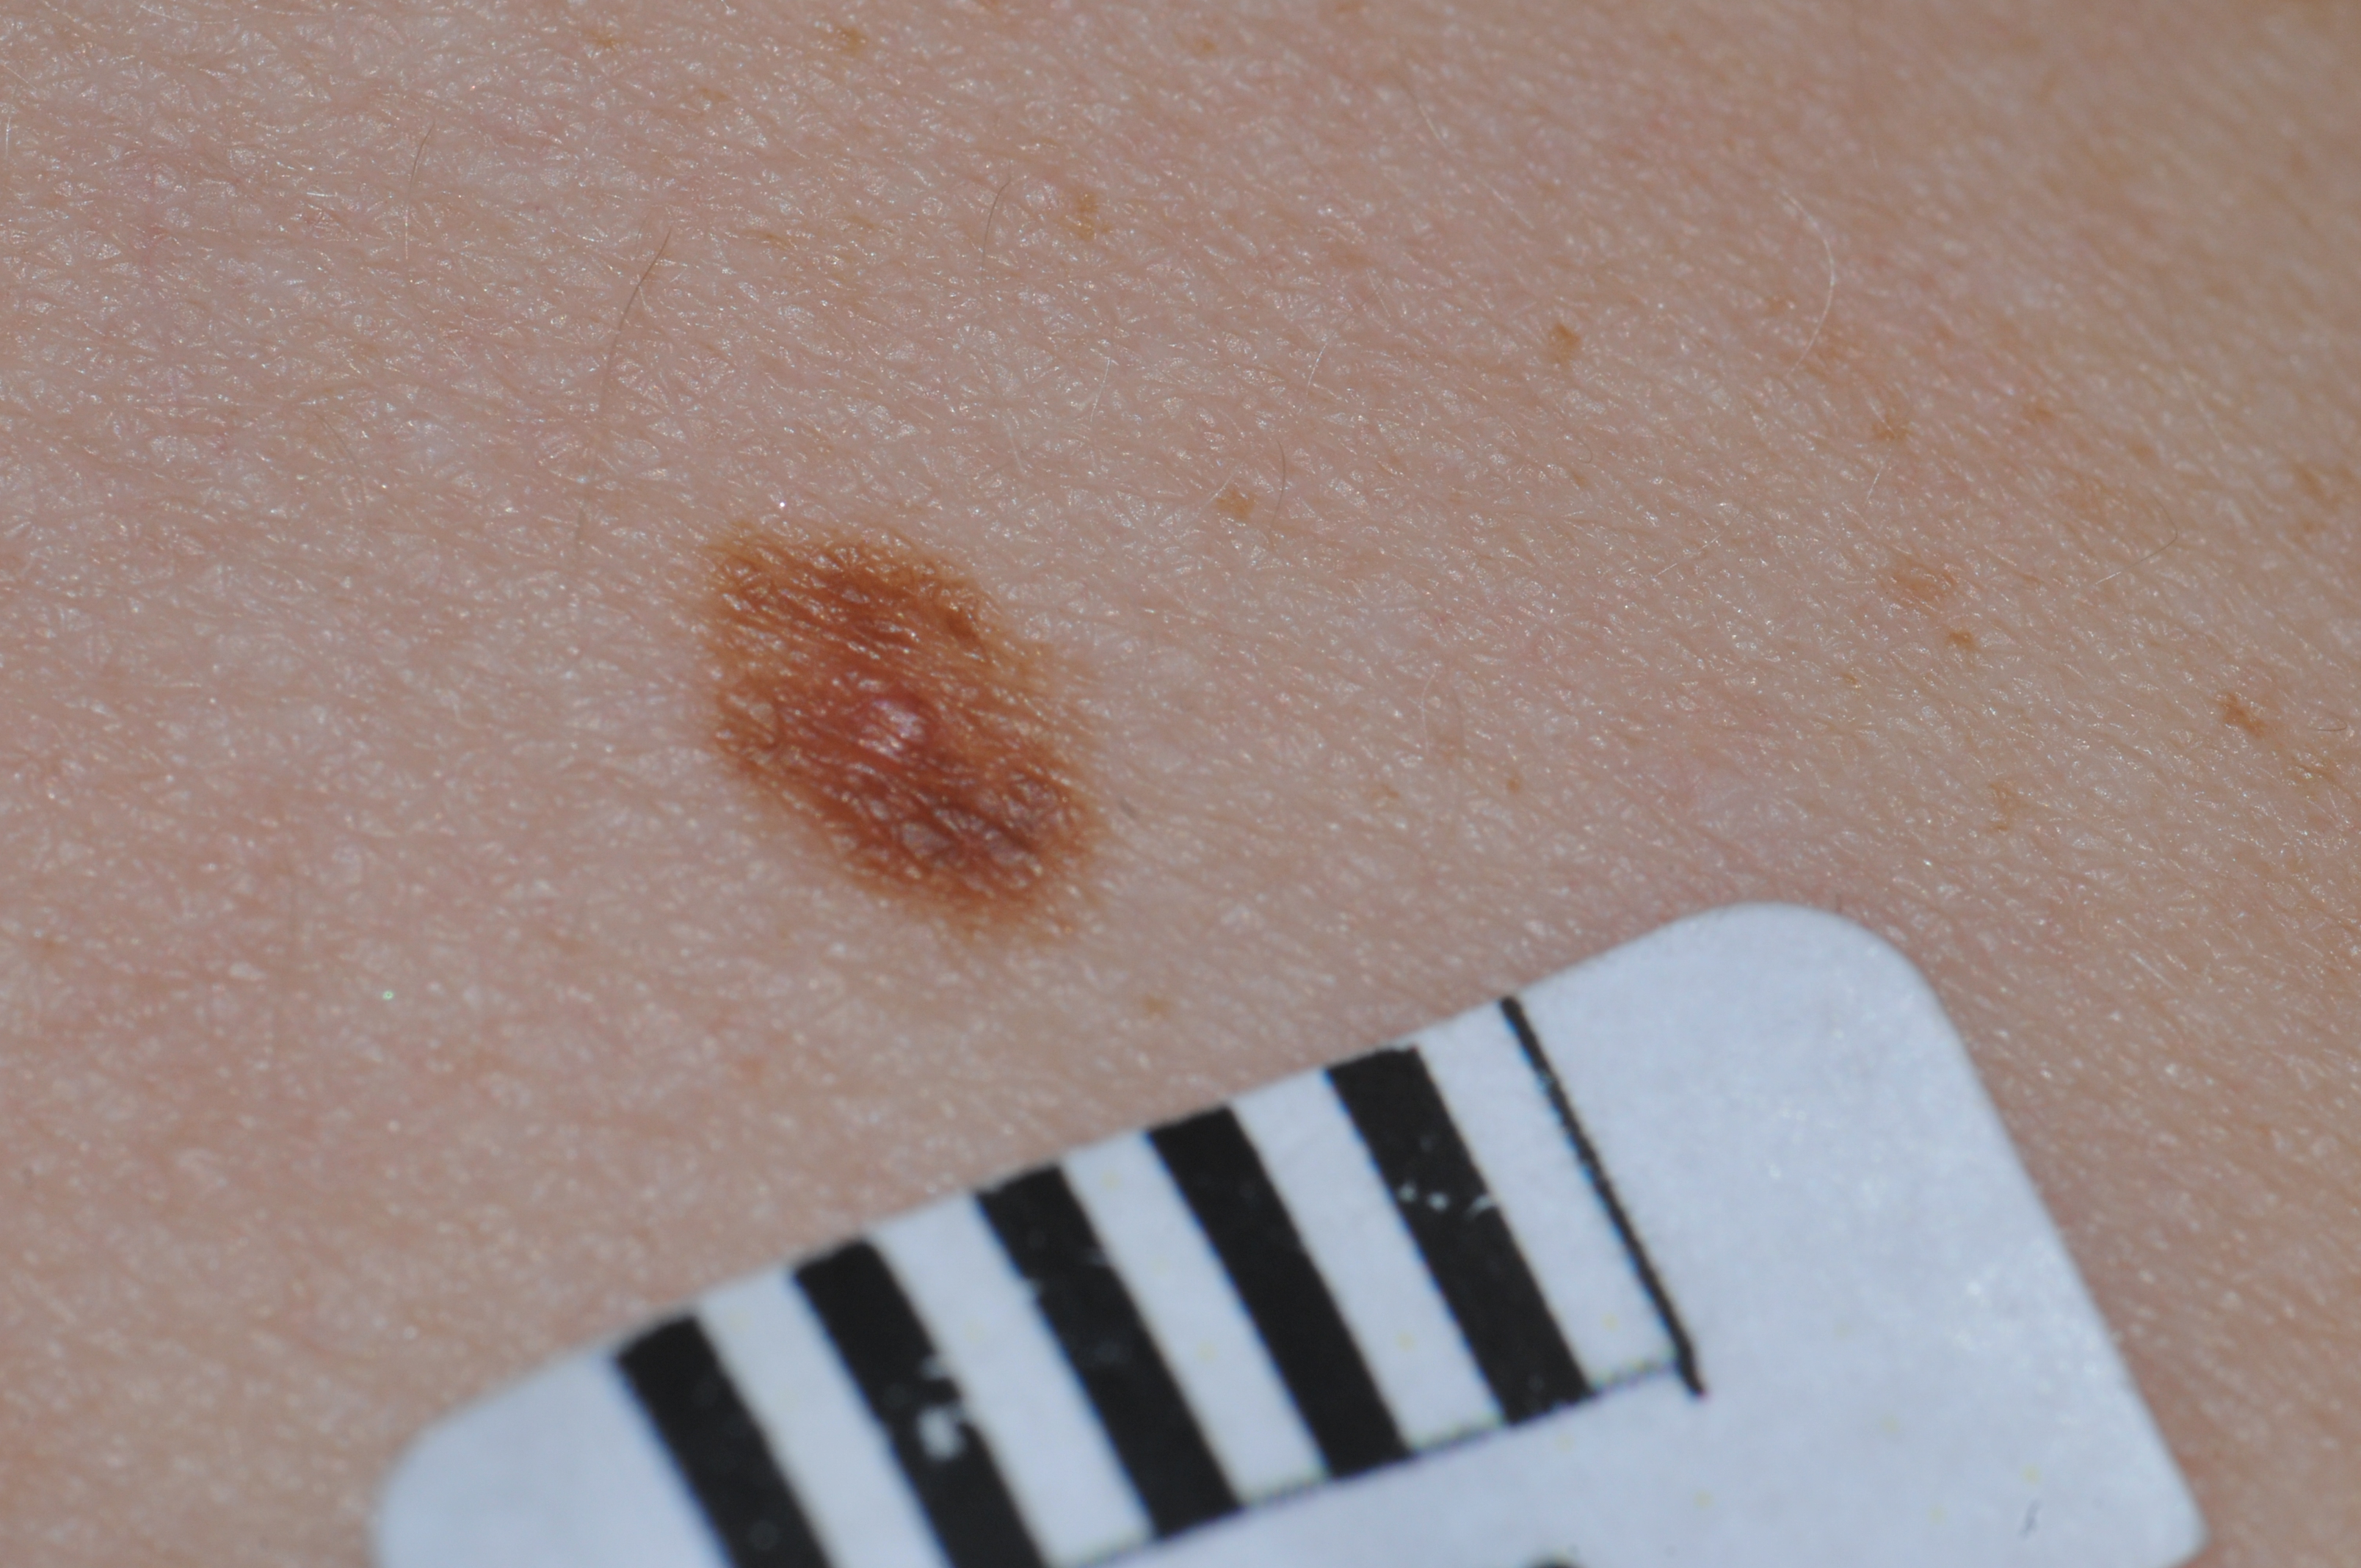
\includegraphics[width=0.3\textwidth]{images/FV_NV.jpg}} &
		\subcaptionbox{\centering Forth Valley Actinic Keratosis}{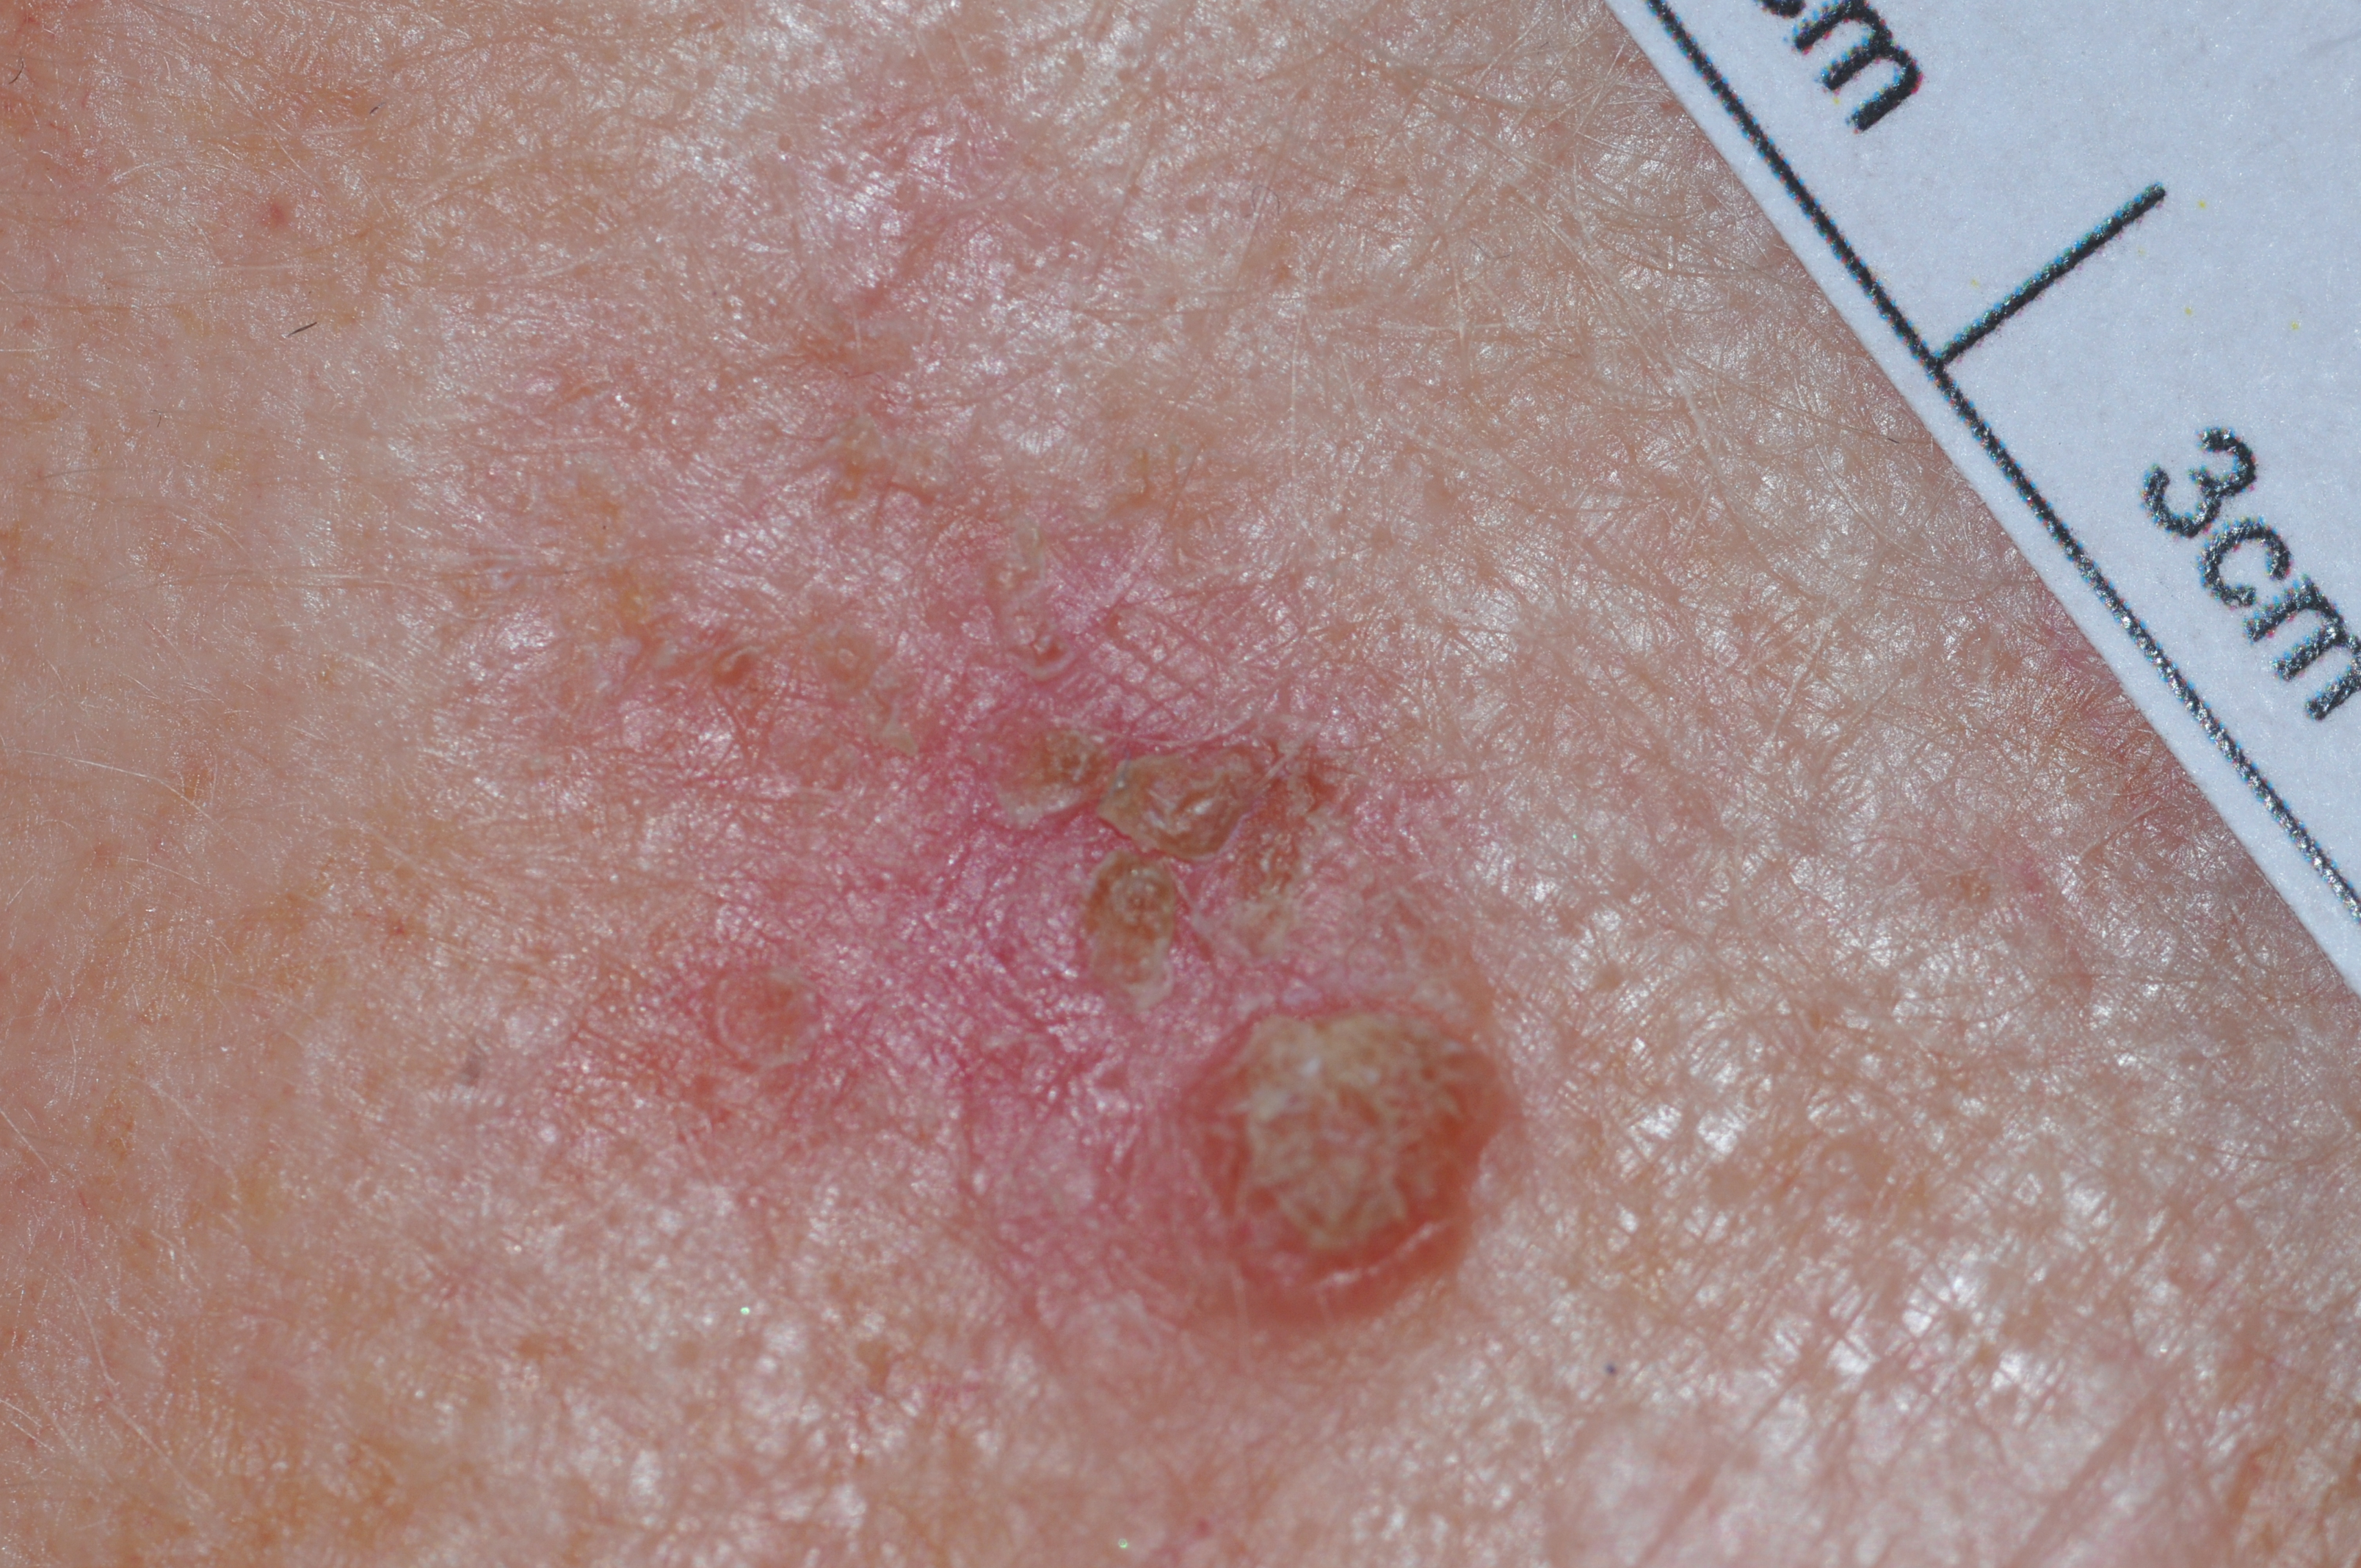
\includegraphics[width=0.3\textwidth]{images/FV_AK.jpg}}
	\end{tabular}
	\caption{Example images from the Tayside and Forth Valley datasets.}
	\label{fig:nhs_dataset_examples}
\end{figure}

\subsection{Tayside Dataset}
\label{subsec:tayside_dataset}
The Tayside dataset (collected by Professor Colin Fleming), sourced from NHS Tayside~\footnote{NHS Tayside: \url{nhstayside.scot.nhs.uk}}, is centred on community-acquired skin lesion data, that represent real-world data capture from primary care. The images were obtained by primary care practitioners utilising a diverse array of cameras, from various cutaneous anatomical sites, utilising non-standardised lighting, framing, focusing, and acquisition settings. The dataset is intended for triage experiments, with the goal of reliably identifying common benign conditions in a real-world clinical setting. This dataset not only represents real-world teledermatology images acquired by primary care practitioners, but it also serves as a proxy for international skin datasets, where high-quality images and dermoscopy may not be readily available.

\subsection{Forth Valley Dataset}
\label{subsec:forth_valley_dataset}
The Forth Valley dataset (collected by Dr. Colin Morton) was procured by medical photographers capturing image of patients skin lesions, who were referred by primary care practitioners for specialist assessment within NHS Forth Valley~\footnote{NHS Forth Valley: \url{nhsforthvalley.com}}. The medical photographers possess a higher degree of expertise in the acquisition of photos of skin lesions, despite potentially lacking specialised knowledge in the field of dermatology. The medical photographers employ standard equipment, such as cameras, lighting, and backgrounds, to ensure uniformity in image quality. Furthermore, a standardised pattern of image capture is utilised to ensure high-quality, wide-angle, and close-up macro images.

\subsection{Annotation Procedure}
\label{subsec:annotation_procedure}
The datasets underwent a comprehensive annotation process that adhered to strict ethical guidelines and protocols for ensuring the quality and clinical usefulness of the images. This annotation procedure was developed by the Dermatology department at NHS Tayside. This included the removal of duplicate images and those that were not clinically relevant, as well as the de-identification and cropping of images to highlight any abnormalities. The images were then assigned a diagnostic label using the British Association of Dermatologists diagnostic index~\footnote{BAD Clinical Guidelines: \url{https://www.bad.org.uk/guidelines-and-standards/clinical-guidelines/}}, which corresponds to the International Classification of Diseases (version 11)~\footnote{ICD-11: \url{https://icd.who.int/dev11/l-derma/en}}. The assignment of these labels was conducted by two consultant-level dermatologists, registered on the UK General Medical Council specialist register of dermatologists~\footnote{UK GMC Medical Register: \url{https://www.gmc-uk.org/registration-and-licensing/the-medical-register/}}, and any discrepancies were resolved by a third consultant-level dermatologist. This decision was based on all available clinical information, including pathology reports from a consultant pathologist. The labels represent real sources of data, with diagnoses for malignancy being derived from pathology, and for benign lesions, based on the opinions of consultant dermatologists. The full annotation procedure is presented in detail for further reference.

\begin{enumerate}
	\item Ensure the necessary Caldicott/Ethical approvals are in place. 
	\item Proceed to open the first patient record.
	\item Proceed to view the images. For each image, determine whether to retain it as potentially diagnostically useful, retain as a negative control, or discard it.
	\begin{enumerate}
		\item Retain as potentially diagnostically useful if any triage-level information can be obtained from the image.
		\item Retain as negative control if a clinical image of skin without even triage level information i.e., where photographic information is insufficient to make a skin diagnosis. This may include images which are blurred by background details e.g., scarring or tattooing.
		\item Discard the image if: a. No skin clinical images present, e.g., a clinical letter with no images may be in your system, X-ray image b. Duplicate image, i.e., multiple images, of which you will choose the best single view.
	\end{enumerate}
	\item If retaining the image, anonymise where necessary. This may involve the removal of distinguishing features e.g., a tattoo, a label with patient details, or full-face views. Minimise cropping to ensure the remaining image has a maximum resolution. 
	\item Where multiple skin lesions, attempt to crop the image to ensure one lesion per image. Minimise cropping to ensure the remaining image has a maximum resolution.
	\item For multiple skin lesions of the same disease process/widespread disease, if not possible to crop sufficiently, ensure all skin lesions have the same diagnostic label and are the same disease process.
	\item Label the image with the diagnosis using BAD Diagnostic Index.
\end{enumerate}


\newpage
\section{Fine-Tuning Experiments}
\label{sec:generalisation_experiments}
This section details the datasets, training parameters, experimental setup, and results for the experiments with dermatology cross dataset fine-tuning. The code and full results used within this section can be found on the project GitHub repository~\footnote{GitHub Repository: \url{github.com/UoD-CVIP/Lesion-Classifier}}.

\subsection{Datasets}
\label{subsec:generalisation_datasets}
In this chapter's experiments, images from two public domain skin lesion datasets are utilised in addition to the datasets from Tayside and Forth Valley. These datasets were the ISIC 2019 dataset~\citep{codella2018skin,combalia2019bcn20000,tschandl2018ham10000} and the SD-260 dataset~\citep{yang2019self}. The ISIC datasets are among the largest publicly available, with ISIC 2019 containing over 26,000 skin lesion images labelled with diagnoses. These images were acquired using dermatoscopes, which tend to produce well-centered, zoomed in, and consistent resolution images. In contrast, the SD-260 images were acquired in less controlled environments with varying imaging devices, resulting in more variation in colour, exposure, illumination, resolution, and scale (Figure~\ref{fig:sd260_examples}). Visually, they are qualitatively similar to the Tayside and Forth Valley datasets but are acquired from a Chinese population.

\begin{figure}
	\centering
	\captionsetup[subfigure]{singlelinecheck=false}
	\begin{tabular}{cc}
		\subcaptionbox{\centering Melanoma}{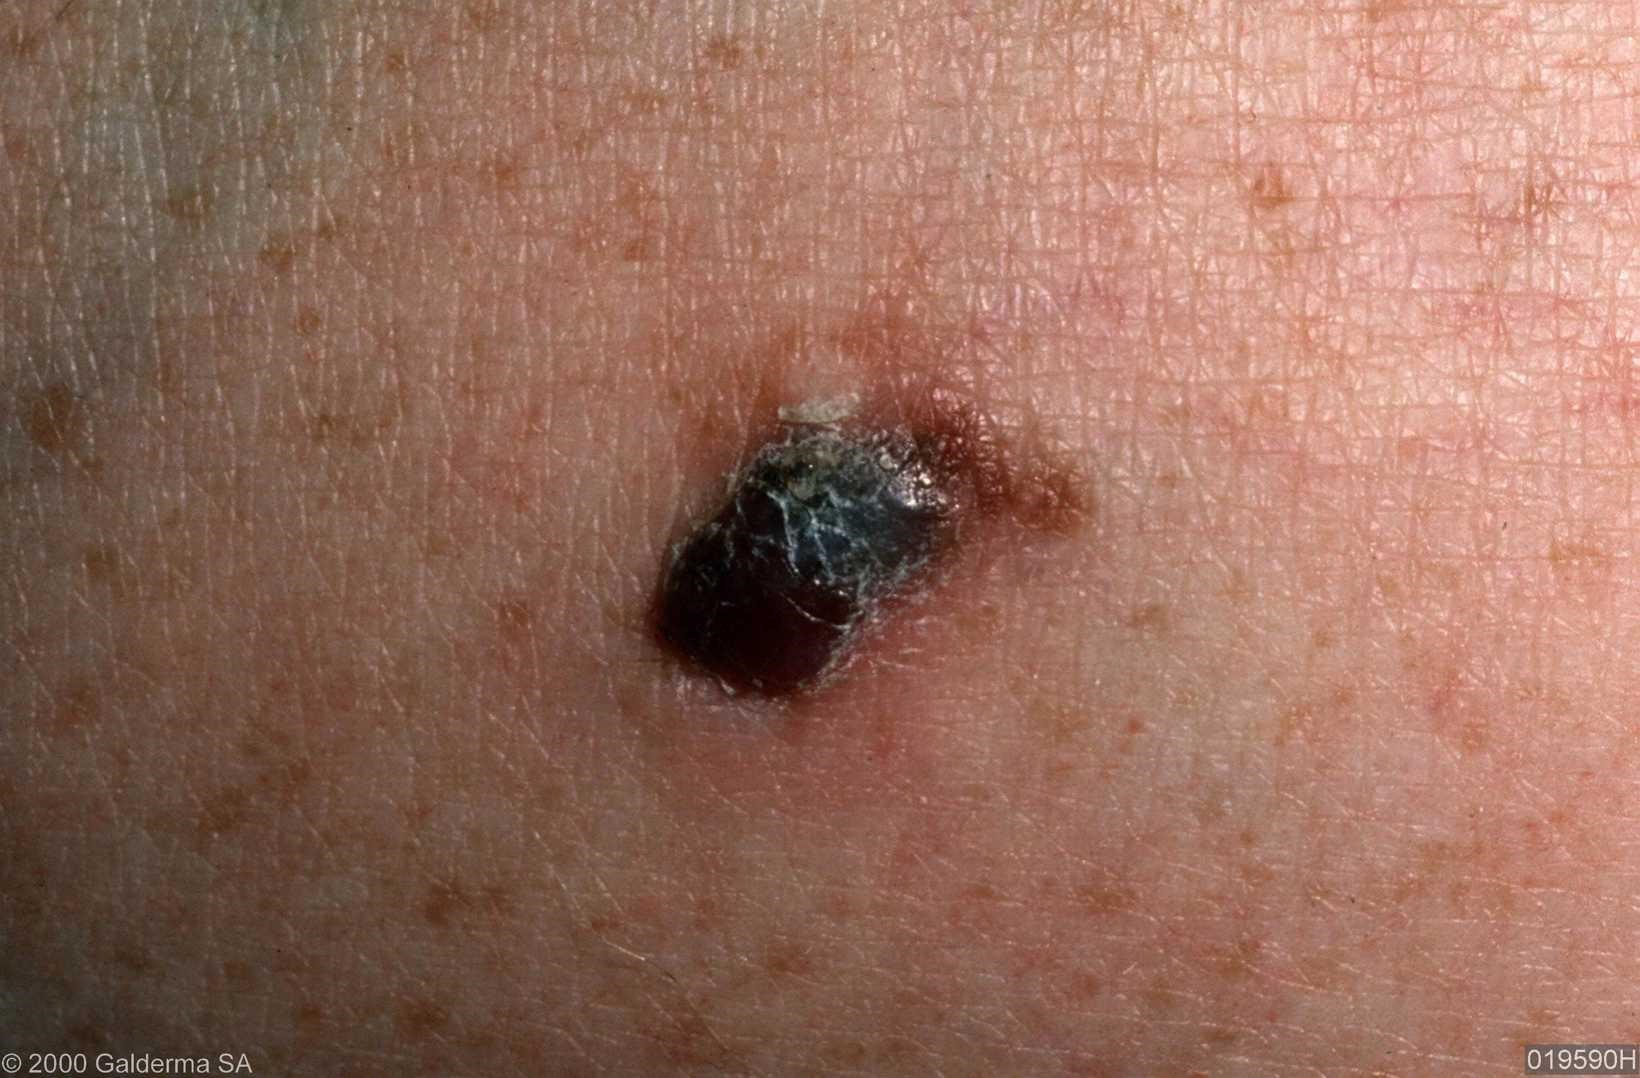
\includegraphics[width=0.45\textwidth]{images/sd260_mel.jpg}} &
		\subcaptionbox{\centering Melanocytic \mbox{Nevus}}{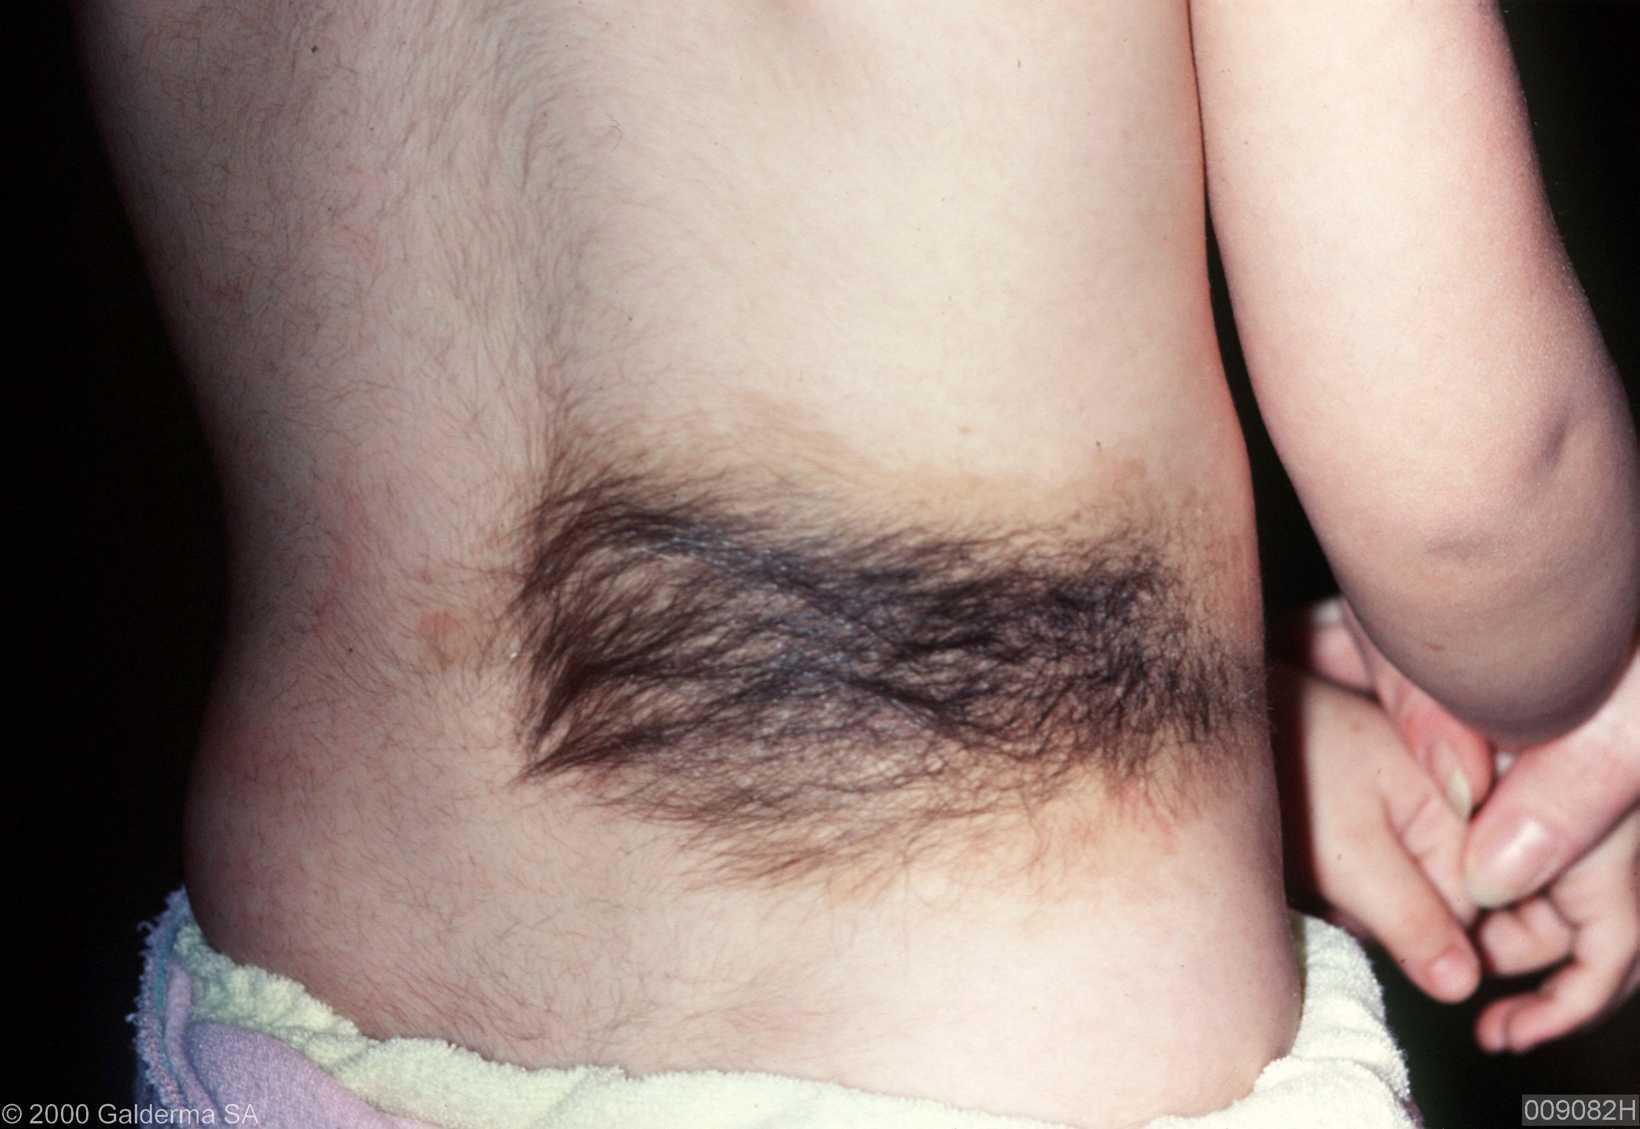
\includegraphics[width=0.45\textwidth]{images/sd260_nv.jpg}} \\
		\subcaptionbox{\centering Basal Cell \mbox{Carcinoma}}{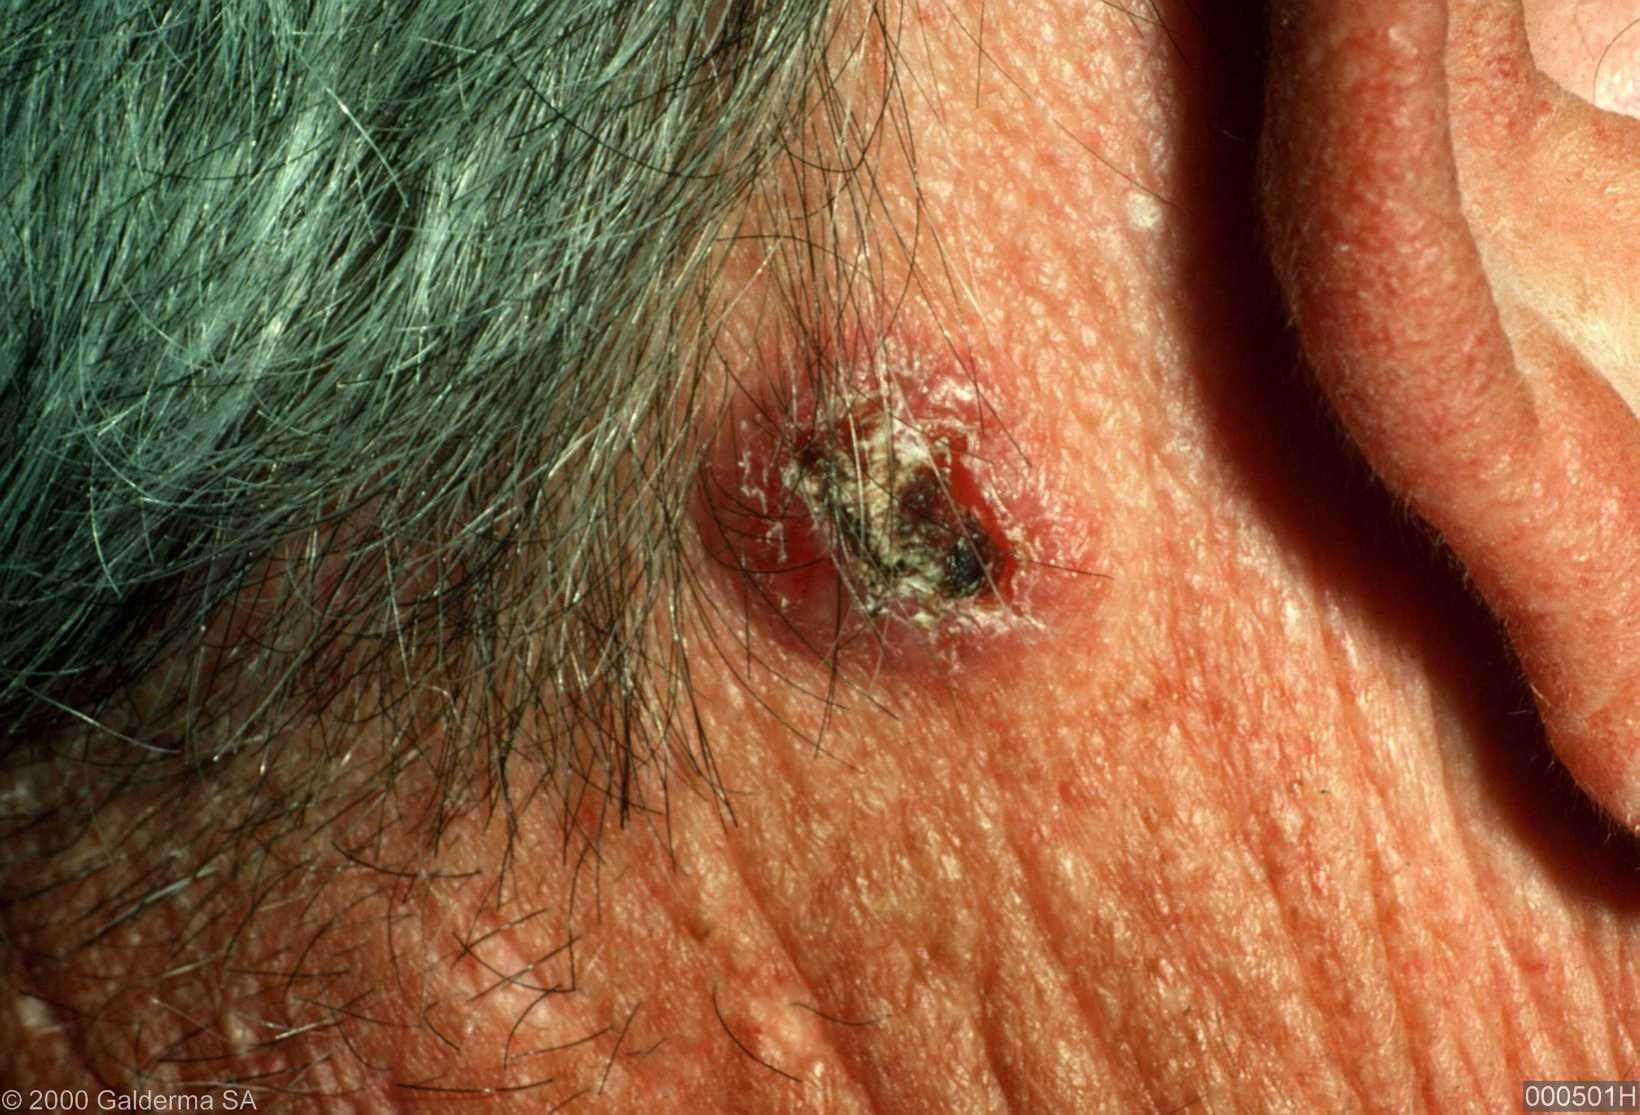
\includegraphics[width=0.45\textwidth]{images/sd260_bcc.jpg}} &
		\subcaptionbox{\centering Actinic Keratosis}{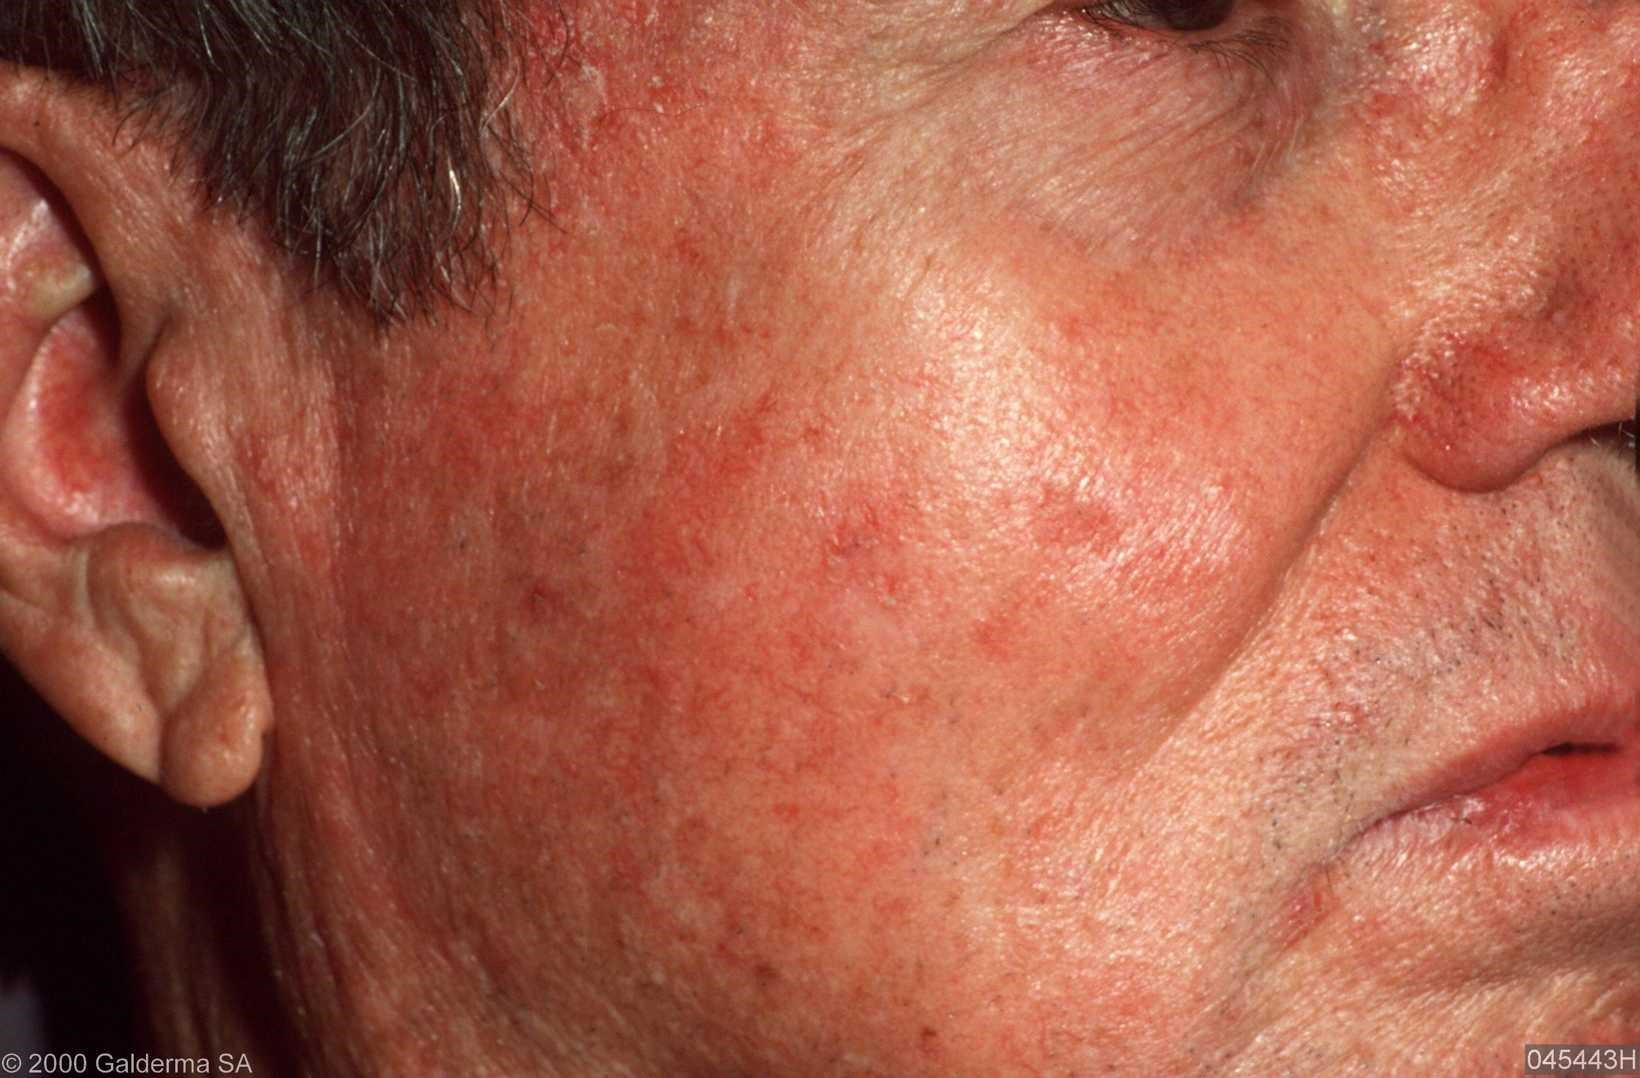
\includegraphics[width=0.45\textwidth]{images/sd260_ak.jpg}} \\
		\subcaptionbox{\centering Benign Keratosis}{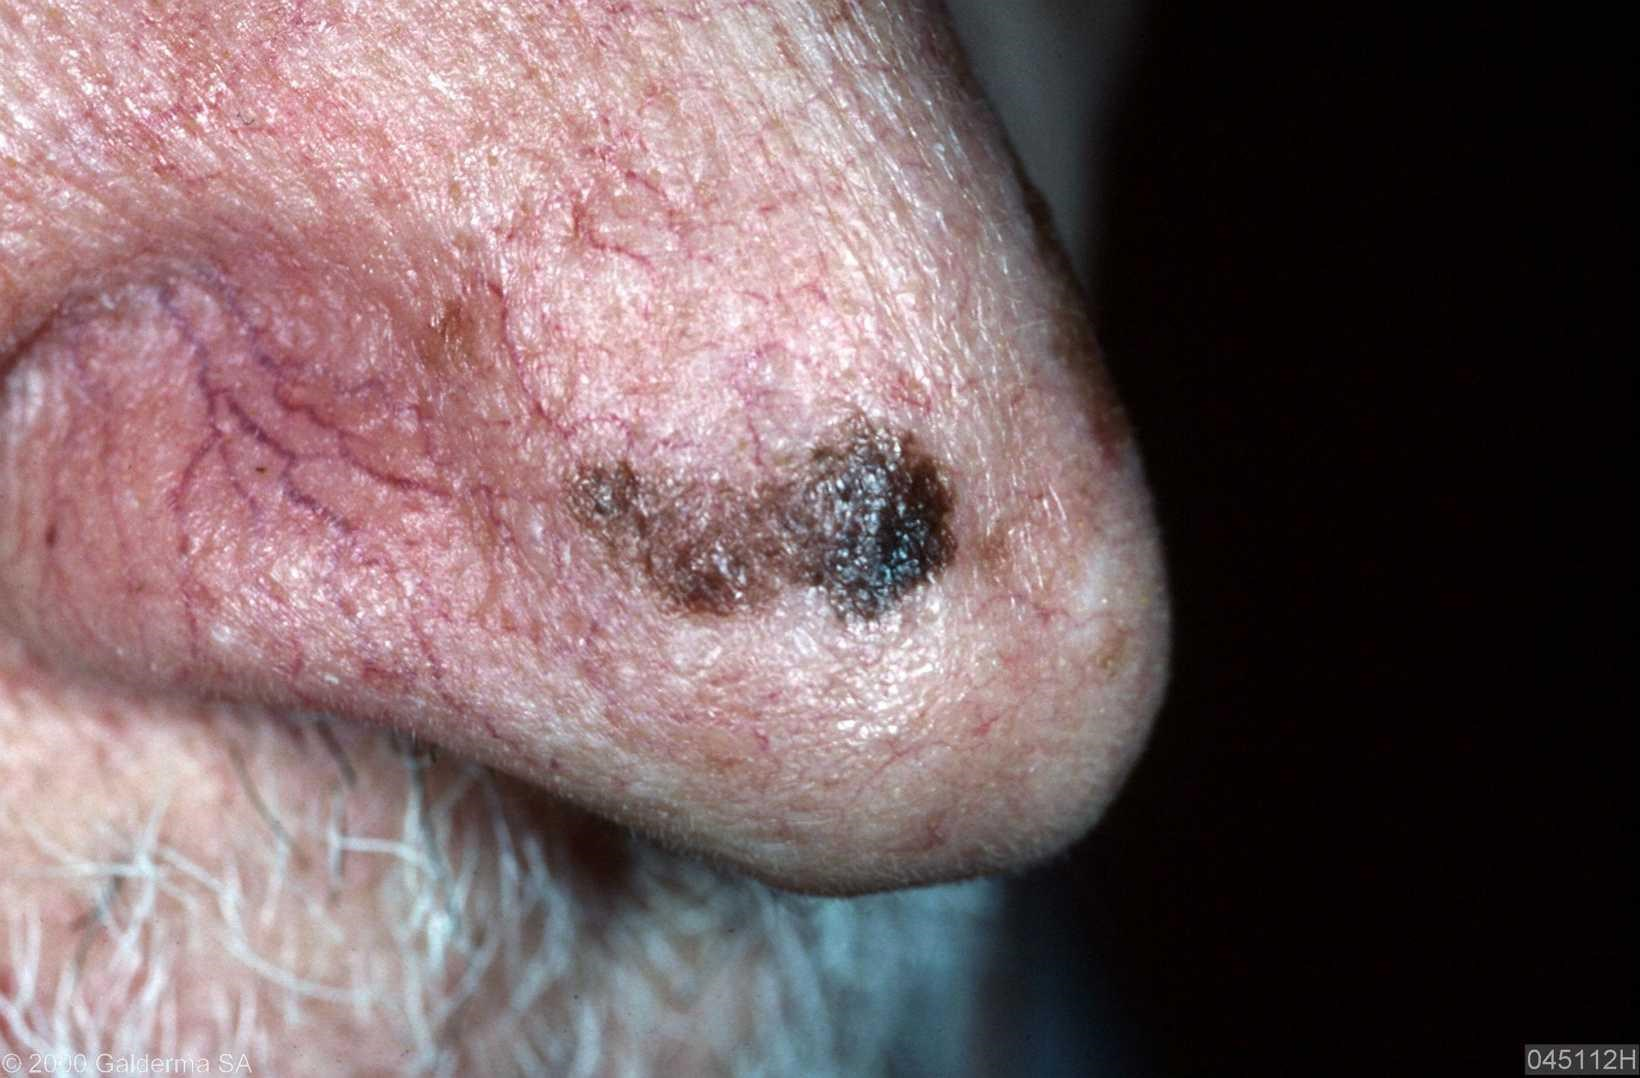
\includegraphics[width=0.45\textwidth]{images/sd260_bkl.jpg}} &
		\subcaptionbox{\centering Dermatofibroma}{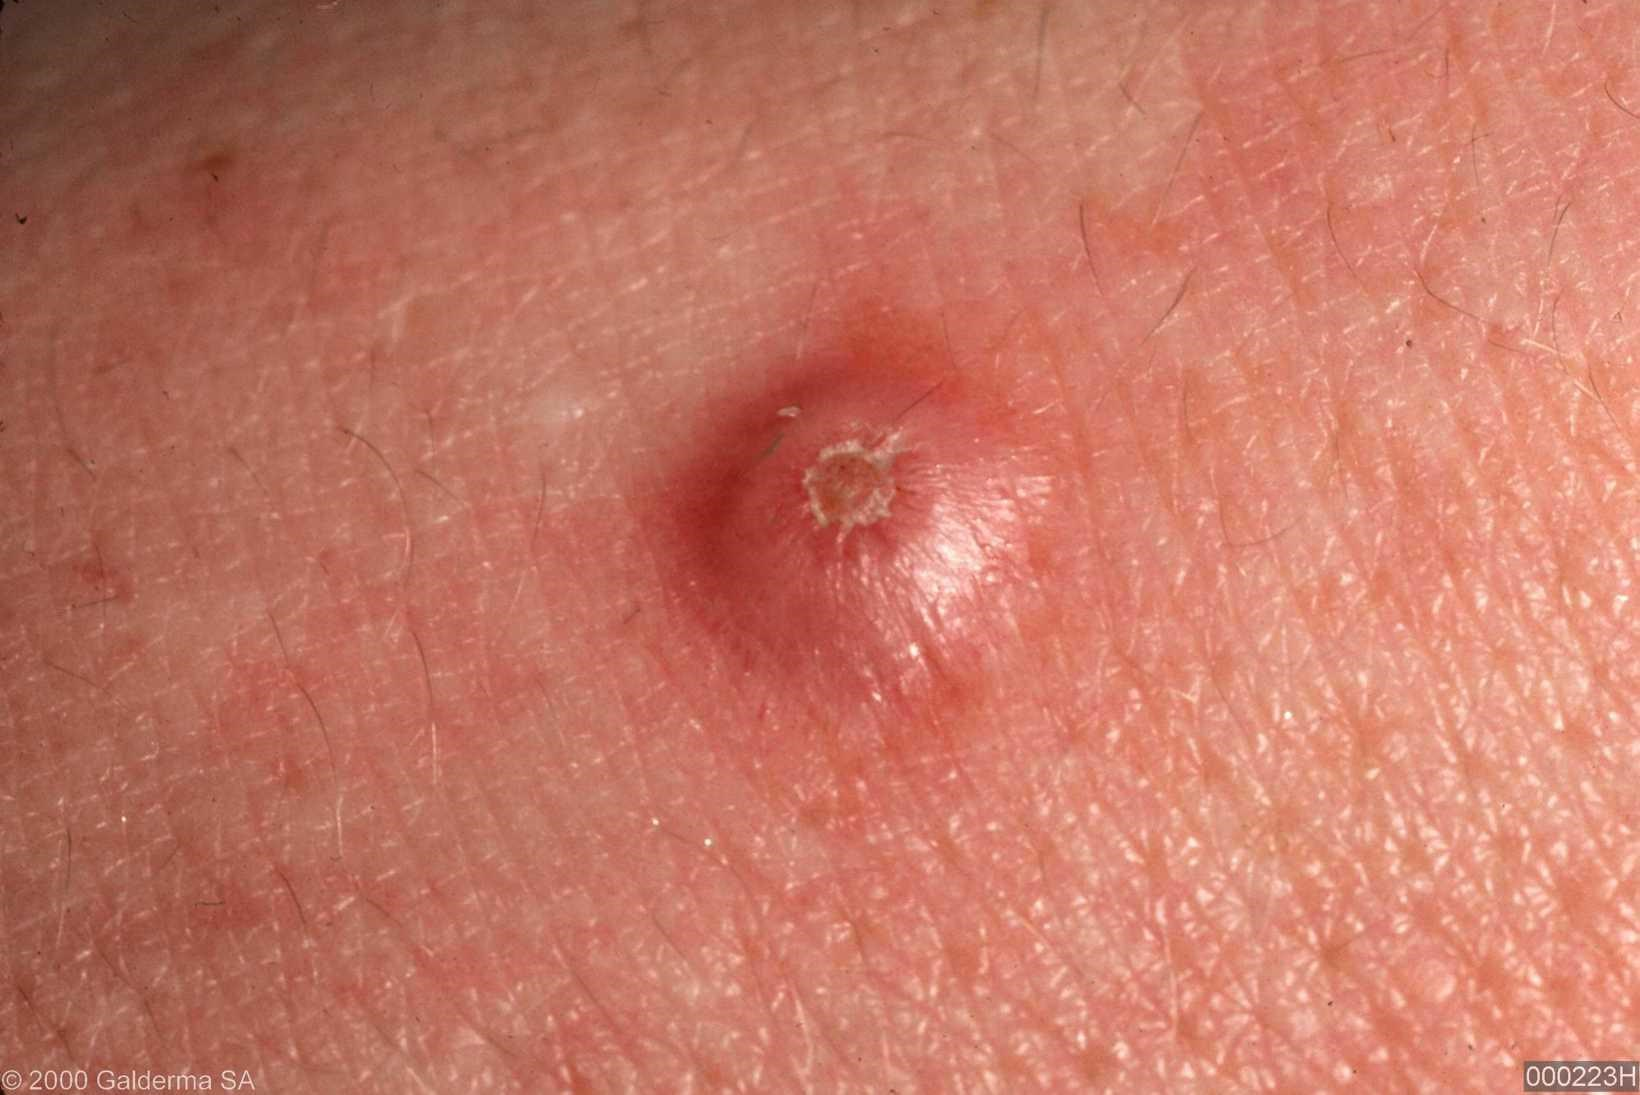
\includegraphics[width=0.45\textwidth]{images/sd260_df.jpg}} \\
		\multicolumn{2}{c}{\subcaptionbox{\centering Squamous Cell \mbox{Carcinoma}}{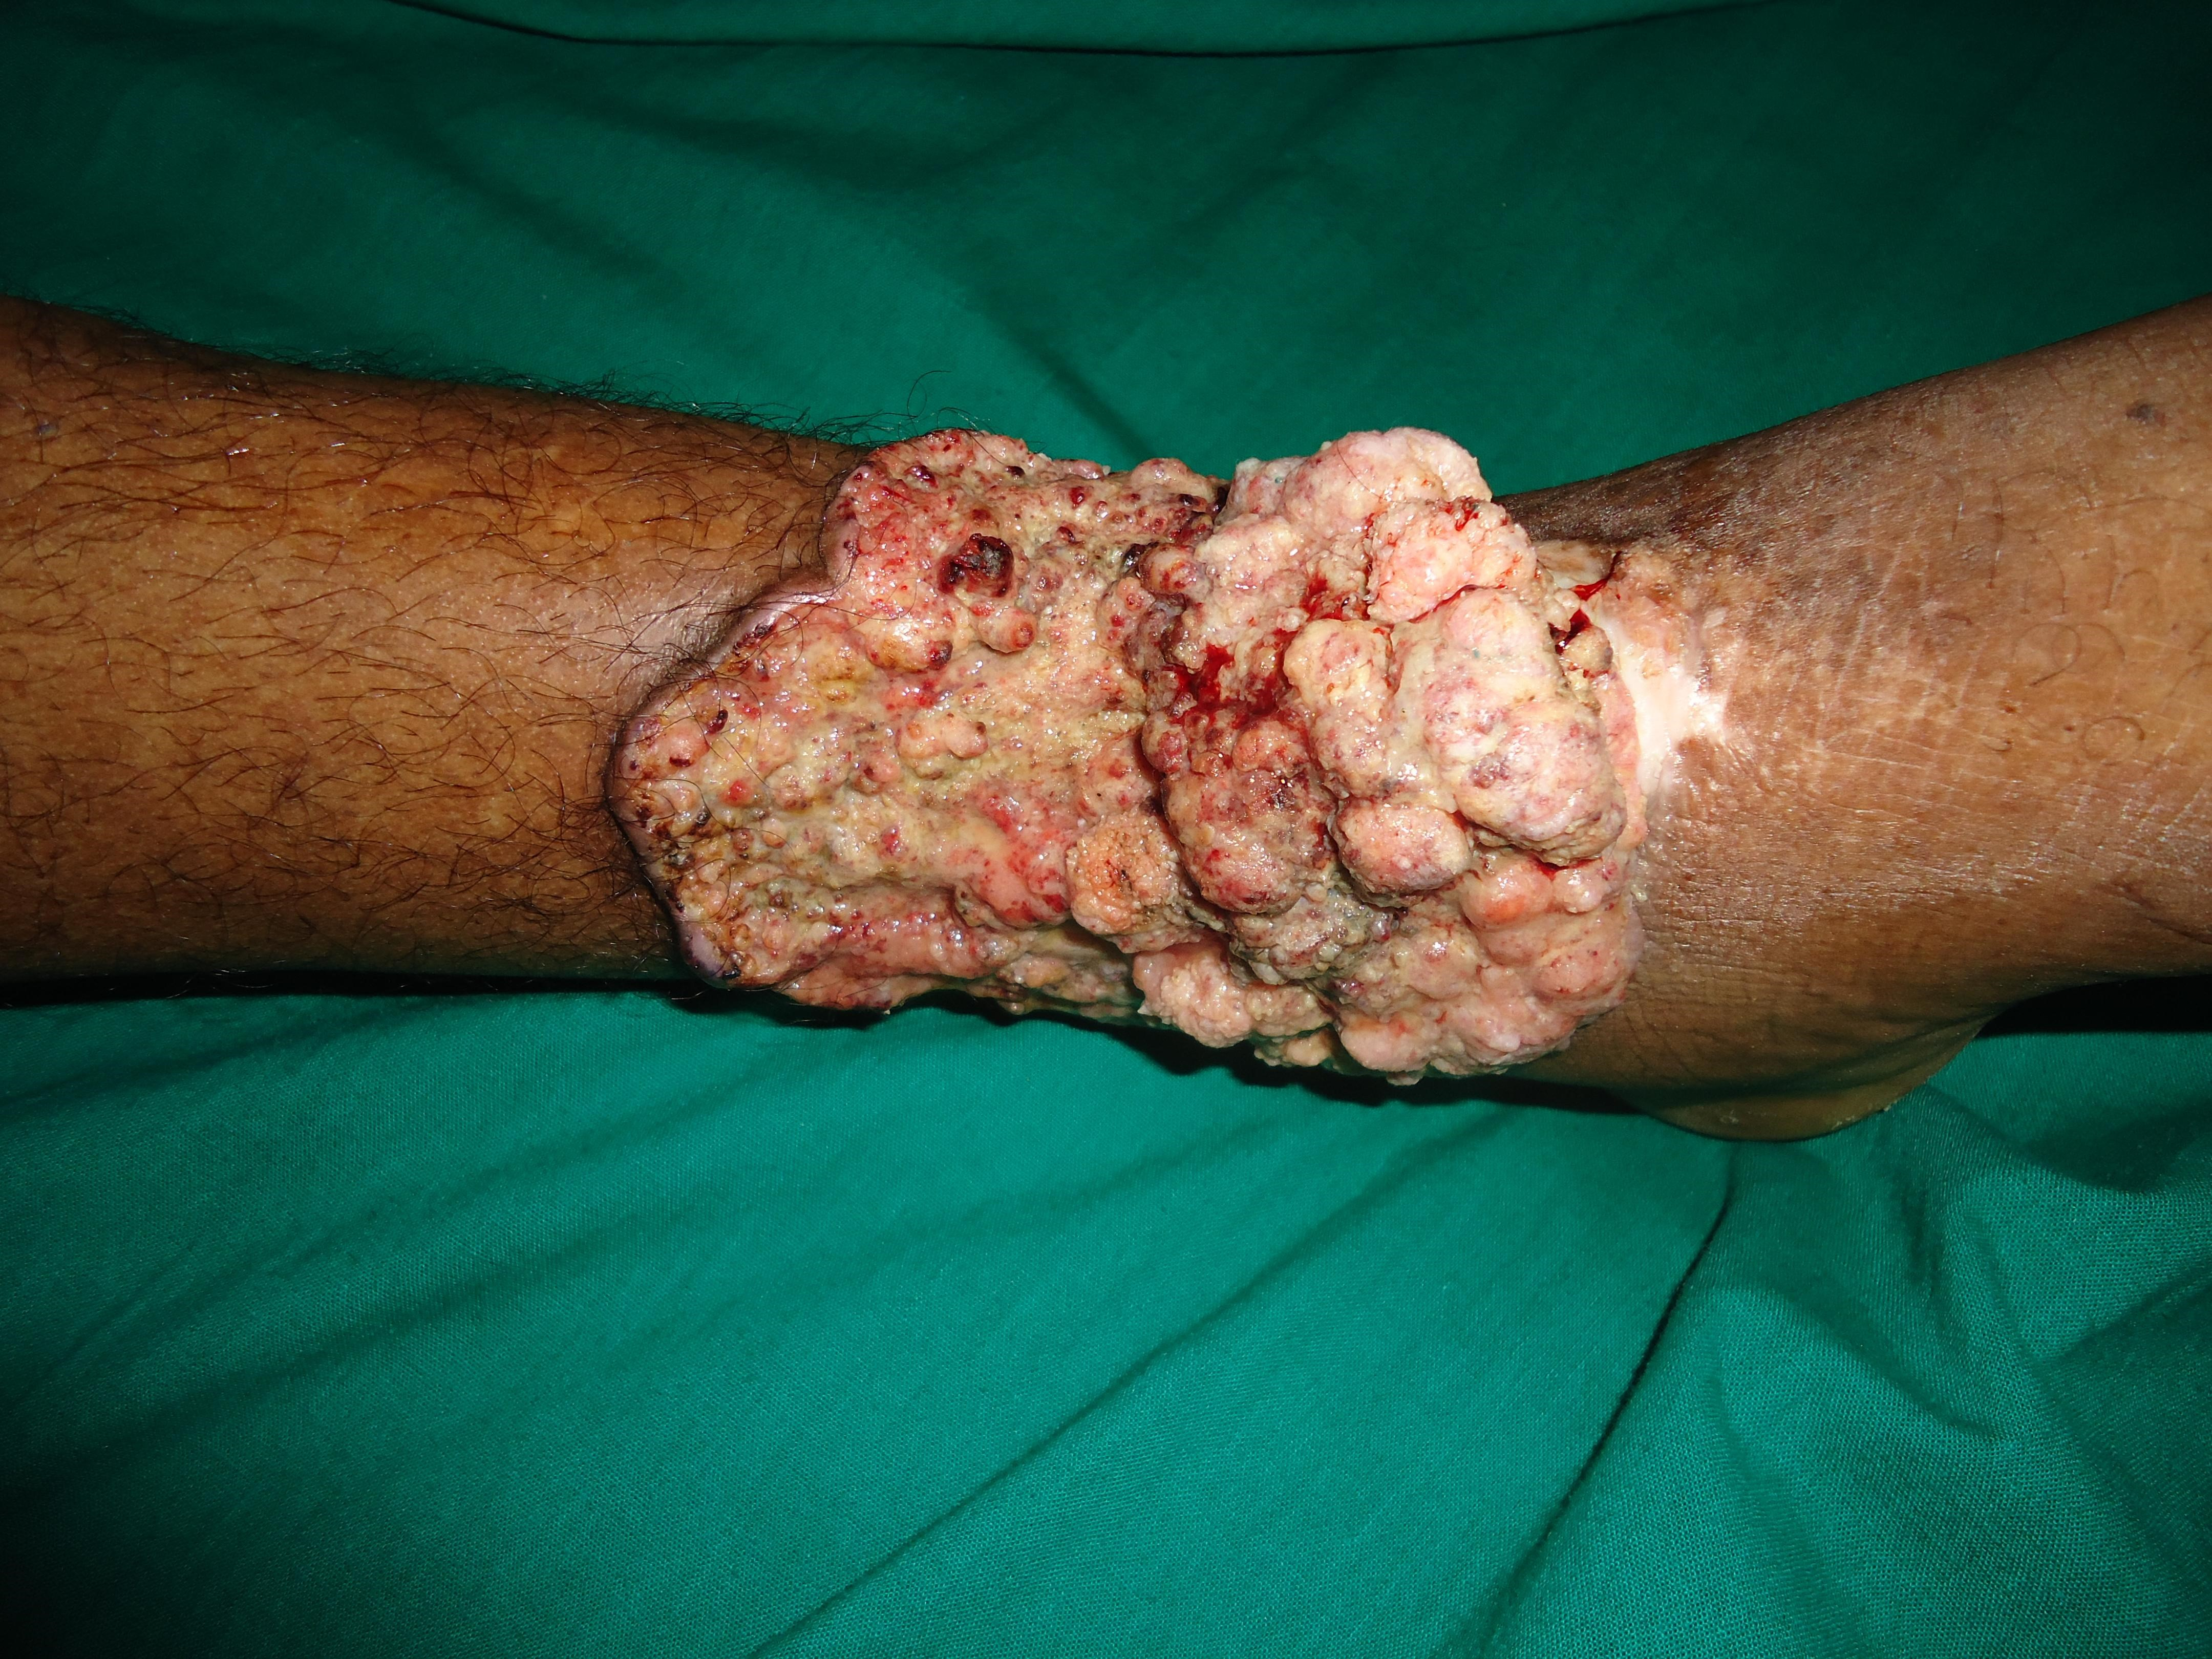
\includegraphics[width=0.45\textwidth]{images/sd260_scc.jpg}}}
	\end{tabular}
	\caption{Example images from the SD-260 dataset~\citep{yang2019self}.}
	\label{fig:sd260_examples}
\end{figure}

To facilitate deep learning experiments, the four skin lesion datasets used in this chapter were intentionally restricted to a set of seven diagnostic categories. The specific seven categories were chosen based on their representation across the four datasets. For example, vascular lesions were excluded from the ISIC 2019 dataset, and classes such as angioma and solar lentigo were excluded from the Tayside dataset because they were not well represented in the other two datasets. The ISIC 2019, SD-260, Tayside, and Forth Valley data subsets used in the chapter contained 25,078, 13,814, 2,213, and 1,510 images, respectively (Table~\ref{tab:generalisation_datasets}).

\begin{table}[h]
	\centering
	\caption{Number of images per diagnosis in each dataset.}
	\label{tab:generalisation_datasets}
	\resizebox{\textwidth}{!}{%
		\begin{tabular}{ll|r|r|r|r|r|}
			\cline{3-7}
			&  & \multicolumn{1}{l|}{ISIC 2019} & \multicolumn{1}{l|}{SD-260} & \multicolumn{1}{l|}{Tayside} & \multicolumn{1}{l|}{Forth Valley} & \multicolumn{1}{l|}{\textit{\textbf{Total}}} \\ \hline
			\multicolumn{1}{|l|}{\multirow{4}{*}{\textbf{Benign}}} & Actinic Keratosis (B52) & 867 & 1,434 & 414 & 143 & \textit{2,858} \\
			\multicolumn{1}{|l|}{} & Dermatofibroma (X9002) & 239 & 303 & 56 & 77 & \textit{675} \\
			\multicolumn{1}{|l|}{} & Naevus, Melanocytic (X31z) & 12,875 & 1,401 & 575 & 530 & \textit{15,381} \\
			\multicolumn{1}{|l|}{} & Seborrhoeic Keratosis (X01) & 2,624 & 1,133 & 537 & 289 & \textit{4,583} \\ \hline
			\multicolumn{1}{|l|}{\multirow{3}{*}{\textbf{Malignant}}} & \begin{tabular}[c]{@{}l@{}}Melanoma (X41) /\\ Melanoma in situ \\ (X40)\end{tabular} & 4,522 & 7,094 & 78 & 204 & \textit{11,898} \\
			\multicolumn{1}{|l|}{} & \begin{tabular}[c]{@{}l@{}}Squamous Cell Carcinoma (X12) /\\ Squamous Cell \\ Carcinoma in situ (X11)\end{tabular} & 628 & 17 & 175 & 89 & \textit{909} \\
			\multicolumn{1}{|l|}{} & Basal Cell Carcinoma (X20) & 3,323 & 2,432 & 378 & 178 & \textit{6,311} \\ \hline
			\multicolumn{2}{|l|}{\textit{\textbf{Total}}} & \textit{25,078} & \textit{13,814} & \textit{2,213} & \textit{1,510} & 42,615 \\ \hline
		\end{tabular}%
	}
\end{table}

\subsection{Training Parameters}
\label{subsec:generalisation_training}
In this chapter, two methods for image classification using deep learning were employed. The first method was a CNN, specifically an EfficientNet architecture~\citep{tan2019efficientnet} with a compound coefficient of 7 and an additional fully connected layer of 512 neurons preceding the output layer. The second method was a SWIN-B transformer~\citep{liu2021swin}, a state-of-the-art visual transformer network for image classification.

Subsequent training sessions were conducted for 40 epochs, with the model being saved each time the lowest validation loss was achieved. The weights were optimised using stochastic gradient descent with batches of 16 images and a triangular$^2$ cyclical scheduler~\citep{smith2017cyclical}, which alternated the learning rate between $10^{-5}$ and $10^{-2}$ and the momentum between 0.8 and 0.9. All images were pre-processed by cropping, resizing to 224 x 224 pixels, and normalising the pixel values between 0.0 and 1.0. To improve fine-tuning generalisation, data augmentation was used, specifically a variety of geometric and photometric changes applied at random when sampling. Horizontal and vertical flips, cropping and padding, affine transforms, Gaussian, average, and median blurring, sharpening, adding to channels, and multiplying channels by arbitrary amounts specifically.

Given an image, the deep network models predicted class probabilities for each of the seven diagnostic classes. These probabilities were constrained, by definition, to sum to one. Three of the seven classes represented malignant lesions. By summing the probabilities of these three classes, the probability that the observed lesion is malignant, assuming the class probabilities computed were well-calibrated (Chapter \ref{ch:classification_claibration}). This was used to evaluate the ability of the EfficientNet CNN and SWIN transformer models to identify malignant lesions. Specifically, ROC curves were used to quantify the sensitivity-specificity trade-offs that can be obtained on the macroscopic image datasets. 

\subsection{Experiment Setup}
\label{subsec:generalisation_experiment}
The ability of the models to classify lesion images from each dataset was first evaluated after training on images from that same dataset. When utilising the larger datasets, ISIC 2019 and SD-260, a disjoint split of 60\% for training, 20\% for validation, and 20\% for testing was employed. These splits were static, and all training and testing with the datasets utilised the same splits. In contrast, given the limited size of the Tayside and Forth Valley datasets, 10-fold cross-validation was utilised to estimate performance, with each fold containing disjoint training (70\%), validation (20\%), and test (10\%) sets. These splits were also static across each fold, with the performance being estimated by averaging the 10 test results.

Subsequently, cross-dataset performance was evaluated by measuring the class-balanced accuracy of each model when tested on data from datasets not used for training the model. Deep classifiers pre-trained with ImageNet~\citep{deng2009imagenet} were trained on data from each of the datasets and then tested on each of the datasets. The composition of the training sets was identical to those used in the internal data classification experiment.

Finally, the effect of transfer learning between the dermatology datasets using an EfficientNet CNN and SWIM transformer models was evaluated. It is noted that all models in the experiments were pre-trained on ImageNet. Further pre-training was then performed on dermatology datasets. The effect of transfer between the large ISIC 2019 and SD-260 datasets was evaluated first. Secondly, the effect of transfer when the target domains (test data) were Tayside and Forth Valley data was investigated, utilising multi-dataset pre-training sequences, such as pre-training on SD-260 data and then training on Forth Valley training data, denoted “SD-260, Forth Valley” or pre-training on ISIC 2019 data, then on SD-260 data, and finally on Tayside training data, denoted “ISIC 2019, SD-260, Tayside”.

Bootstrapping is used to evaluate model performance (100 bootstraps were sampled); mean class accuracy is obtained for each bootstrap, and the average mean class accuracy is presented together with the 95\% confidence and 95\% tolerance intervals (intervals within which 95\% of bootstrapped test results lie). To describe the sensitivity-specificity trade-offs obtained when categorising test pictures as benign or malignant, ROC curves were constructed.


\subsection{Results}
\label{subsec:generalisation_results}
Table~\ref{tab:generalisation_results} presents the balanced class accuracies obtained using an EfficientNet CNN and SWIN transformer models when trained and tested on data from the four datasets. The diagonal entries, in bold, reflect the internal accuracies obtained when disjoint test and training sets from the same source dataset were used. The results of models trained using the comparably smaller NHS datasets and then tested against the larger datasets were excluded from these experiments. This omission is due to the result not being necessary for the primary objective of this work, which is to examine the results when the models are tested against the moderately sized NHS datasets.

\begin{table}[th]
	\centering
	\caption{Mean class accuracy test results for EfficientNet CNN and SWIN classifiers trained on each of the four datasets. Bootstrapped 95\% confidence intervals are in parentheses.}
	\label{tab:generalisation_results}
	\resizebox{\textwidth}{!}{%
		\begin{tabular}{ll|rrrr|}
			\cline{3-6}
			&  & \multicolumn{4}{c|}{Testing Dataset} \\ \hline
			\multicolumn{1}{|c|}{Model} & \multicolumn{1}{c|}{Training Dataset} & \multicolumn{1}{c|}{ISIC 2019} & \multicolumn{1}{c|}{SD-260} & \multicolumn{1}{c|}{Tayside} & \multicolumn{1}{c|}{Forth Valley} \\ \hline
			\multicolumn{1}{|l|}{\multirow{4}{*}{\textbf{CNN}}} & ISIC 2019 & \multicolumn{1}{r|}{{$\boldsymbol{0.975\, (\pm0.0002)}$}} & \multicolumn{1}{r|}{$0.810\, (\pm0.0007)$} & \multicolumn{1}{r|}{$0.823\, (\pm0.0006)$} & $0.850\, (\pm0.0007)$ \\
			\multicolumn{1}{|l|}{} & SD-260 & \multicolumn{1}{r|}{$0.875\, (\pm0.0004)$} & \multicolumn{1}{r|}{$\boldsymbol{0.957\, (\pm0.0005)}$} & \multicolumn{1}{r|}{$0.852\, (\pm0.0006)$} & $0.871\, (\pm0.0006)$ \\
			\multicolumn{1}{|l|}{} & Tayside & \multicolumn{1}{r|}{} & \multicolumn{1}{r|}{} & \multicolumn{1}{r|}{$\boldsymbol{0.881\, (\pm0.0006)}$} & $0.857\, (\pm0.0002)$ \\
			\multicolumn{1}{|l|}{} & Forth Valley & \multicolumn{1}{r|}{} & \multicolumn{1}{r|}{} & \multicolumn{1}{r|}{$0.846\, (\pm0.0002)$} & $\boldsymbol{0.891\, (\pm0.0007)}$ \\ \hline
			\multicolumn{1}{|l|}{\multirow{4}{*}{\textbf{SWIN}}} & ISCI 2019 & \multicolumn{1}{r|}{$\boldsymbol{0.978\, (\pm0.0002)}$} & \multicolumn{1}{r|}{$0.788\, (\pm0.0006)$} & \multicolumn{1}{r|}{$0.812\, (\pm0.0005)$} & $0.853\, (\pm0.0008)$ \\
			\multicolumn{1}{|l|}{} & SD-260 & \multicolumn{1}{r|}{$0.880\, (\pm0.0004)$} & \multicolumn{1}{r|}{$\boldsymbol{0.971\, (\pm0.0005)}$} & \multicolumn{1}{r|}{$0.859\, (\pm0.0006)$} & $0.870\, (\pm0.0007)$ \\
			\multicolumn{1}{|l|}{} & Tayside & \multicolumn{1}{r|}{} & \multicolumn{1}{r|}{} & \multicolumn{1}{r|}{$\boldsymbol{0.876\, (\pm0.0007)}$} & $0.864\, (\pm0.0002)$ \\
			\multicolumn{1}{|l|}{} & Forth Valley & \multicolumn{1}{r|}{} & \multicolumn{1}{r|}{} & \multicolumn{1}{r|}{$0.850\, (\pm0.0002)$} & $\boldsymbol{0.898\, (\pm0.0007)}$ \\ \hline
		\end{tabular}%
	}
\end{table}

Overall, in the absence of training data from the target domains, training on SD-260 data provided the best test accuracies on all test datasets. Models trained on ISIC data did not generalise well to the other datasets, while models trained on SD-260 data generalised slightly better but still poorly. Fine-tuning generalisation between the Tayside and Forth Valley datasets was better, with relatively small drops in test accuracy. Models trained on Tayside data achieved test results on Forth Valley data only 2.4\% and 1.2\% lower than test results on Tayside data.

Additionally, it was observed that models trained and tested on ISIC data did not benefit from pre-training on SD-260; ISIC test results with SD-260 pre-training were 98.5\% and 98.5\% for EfficientNet CNN and SWIN, respectively. Similarly, models trained and tested on SD-260 data did not benefit from pre-training on ISIC data. SD-260 test results with ISIC pre-training were 97.2\% and 96.2\% for EfficientNet CNN and SWIN, respectively.

This occurrence may be linked to the appearance of negative transfer, in which traits gained during the initial ISIC pre-training phase may have deleterious consequences when applied to the subsequent SD-260 training regimen. As indicated by the existing literature~\citep{wang2019characterizing}, negative transfer can be caused by a variety of causes, including inconsistencies in feature alignment, discordant patterning, instances of overfitting, and, most significantly, domain shift. In this specific context, the perceptible disparity in the relevance of knowledge gained from the ISIC domain versus its application to the SD-260 training domain may underpin the emergence of optimisation challenges, potentially culminating in entrapment within local minima configurations.

Table~\ref{tab:generalisation_models} reports balanced class accuracies when EfficientNet CNN and SWIN transformers were tested on Tayside and Forth Valley data after various multi-dataset training sequences. In each case, pre-training on SD-260 data followed by fine-tuning on data from the target domain was found to be effective.

\begin{table}[t]
	\centering
	\caption{Mean class accuracy for EfficientNet CNN and SWIN classifiers tested on Tayside and Forth Valley data having been trained with various multi-dataset training sequences. 95\% confidence intervals are in parentheses.}
	\label{tab:generalisation_models}
	\resizebox{\textwidth}{!}{%
		\begin{tabular}{ll|rr|}
			\cline{3-4}
			&  & \multicolumn{2}{l|}{Testing Datasets} \\ \hline
			\multicolumn{1}{|l|}{Model} & Training Datasets & \multicolumn{1}{l|}{Tayside} & \multicolumn{1}{l|}{Forth Valley} \\ \hline
			\multicolumn{1}{|l|}{\multirow{8}{*}{\textbf{CNN}}} & SD-260, ISIC 2019 & \multicolumn{1}{r|}{$0.827\,(\pm0.0007)$} & $0.847\,(\pm0.0007)$ \\
			\multicolumn{1}{|l|}{} & ISIC 2019, SD-260 & \multicolumn{1}{r|}{$0.855\,(\pm0.0006)$} & $0.871\,(\pm0.0008)$ \\
			\multicolumn{1}{|l|}{} & ISIC 2019, Tayside & \multicolumn{1}{r|}{$0.877\,(\pm0.0006)$} & $0.875\,(\pm0.0002)$ \\
			\multicolumn{1}{|l|}{} & SD-260, Tayside & \multicolumn{1}{r|}{$\boldsymbol{0.885\,(\pm0.0006)}$} & $0.877\,(\pm0.0003)$ \\
			\multicolumn{1}{|l|}{} & ISIC 2019, SD-260, Tayside & \multicolumn{1}{r|}{$0.880\,(\pm0.0006)$} & $0.869\,(\pm0.0002)$ \\
			\multicolumn{1}{|l|}{} & ISIC 2019, Forth Valley & \multicolumn{1}{r|}{$0.851\,(\pm0.0002)$} & $0.904\,(\pm0.0007)$ \\
			\multicolumn{1}{|l|}{} & SD-260, Forth Valley & \multicolumn{1}{r|}{$0.861\,(\pm0.0002)$} & $\boldsymbol{0.905\,(\pm0.0007)}$ \\
			\multicolumn{1}{|l|}{} & ISIC 2019, SD-260, Forth Valley & \multicolumn{1}{r|}{$0.850\,(\pm0.0002)$} & $0.896\,(\pm0.0007)$ \\ \hline
			\multicolumn{1}{|l|}{\multirow{8}{*}{\textbf{SWIN}}} & SD-260, ISIC 2019 & \multicolumn{1}{r|}{$0.833\,(\pm0.0005)$} & $0.870\,(\pm0.0007)$ \\
			\multicolumn{1}{|l|}{} & ISIC 2019, SD-260 & \multicolumn{1}{r|}{$0.856\,(\pm0.0006)$} & $0.874\,(\pm0.0008)$ \\
			\multicolumn{1}{|l|}{} & ISIC 2019, Tayside & \multicolumn{1}{r|}{$0.881\,(\pm0.0006)$} & $0.878\,(\pm0.0002)$ \\
			\multicolumn{1}{|l|}{} & SD-260, Tayside & \multicolumn{1}{r|}{$\boldsymbol{0.885\,(\pm0.0006)}$} & $0.882\,(\pm0.0002)$ \\
			\multicolumn{1}{|l|}{} & ISIC 2019, SD-260, Tayside & \multicolumn{1}{r|}{$0.883\,(\pm0.0007)$} & $0.888\,(\pm0.0007)$ \\
			\multicolumn{1}{|l|}{} & ISIC 2019, Forth Valley & \multicolumn{1}{r|}{$0.856\,(\pm0.0002)$} & $0.905\,(\pm0.0007)$ \\
			\multicolumn{1}{|l|}{} & SD-260, Forth Valley & \multicolumn{1}{r|}{$0.862\,(\pm0.0002)$} & $\boldsymbol{0.911\,(\pm0.0007)}$ \\
			\multicolumn{1}{|l|}{} & ISIC 2019, SD-260, Forth Valley & \multicolumn{1}{r|}{$0.857\,(\pm0.0002)$} & $0.908\,(\pm0.0008)$ \\ \hline
		\end{tabular}%
	}
\end{table}

\begin{figure}[!th]
	\centering
	\captionsetup[subfigure]{singlelinecheck=false}
	\begin{tabular}{c}
		\subcaptionbox{\centering Testing on the Tayside dataset.}{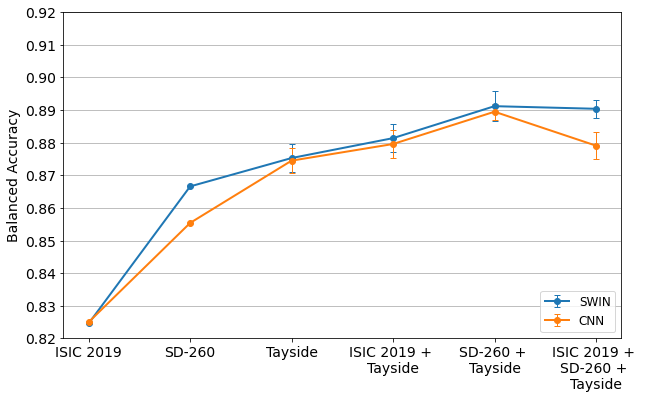
\includegraphics[width=\textwidth]{images/tayside_model.png}} \\
		\subcaptionbox{\centering Testing on the Forth Valley dataset.}{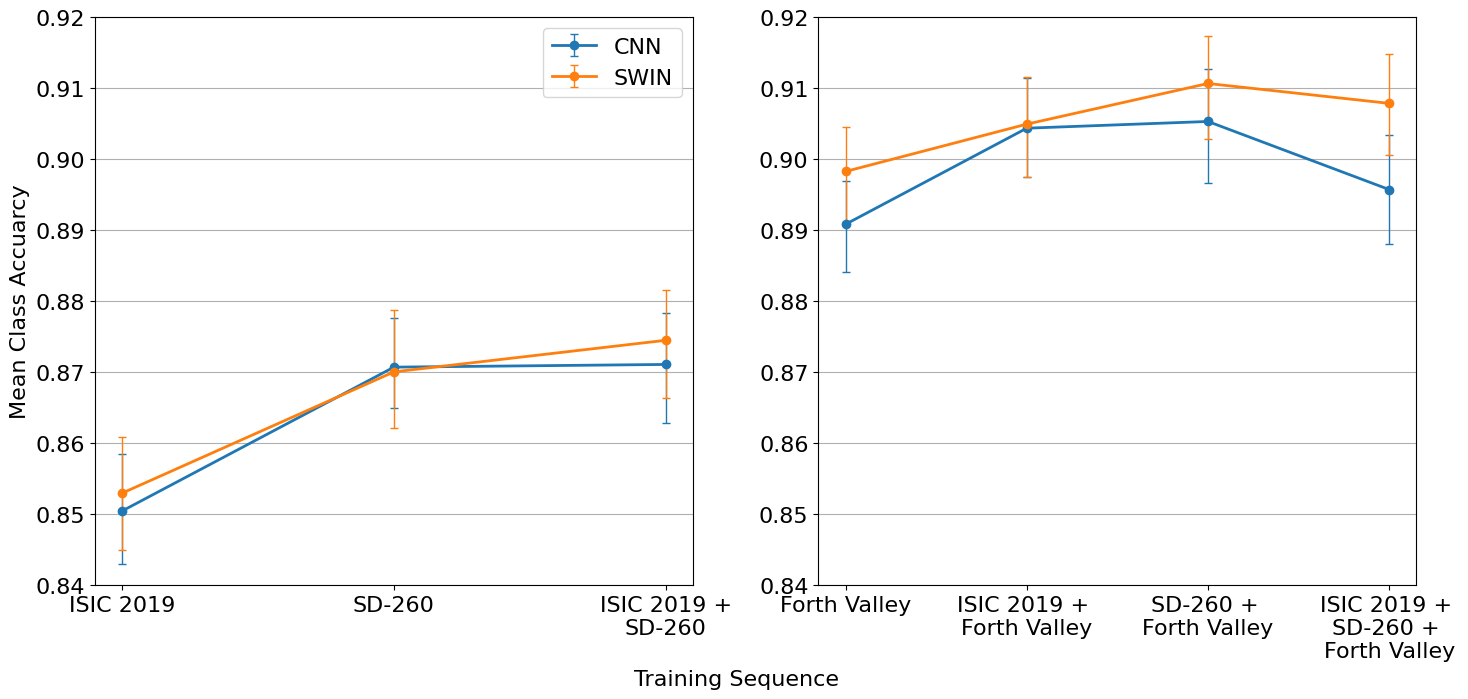
\includegraphics[width=\textwidth]{images/forth_valley_model.png}}
	\end{tabular}
	\caption{Mean class accuracy results for EfficientNet CNN (blue) and SWIN (orange) benign-malignant classifiers tested on (a) Tayside and (b) Forth Valley data. Bars indicate 95\% tolerance intervals computed using bootstrap. The plots on the left are from classifiers trained only on public domain datasets. The plots on the right are cross-validation results from classifiers pre-trained using public domain datasets and then fine-tuned using data from the target domain, i.e., Tayside and Forth Valley, respectively.}
	\label{fig:generalisation_models}
\end{figure}

The results are also illustrated in Figure~\ref{fig:generalisation_models} which shows how test accuracies changed when different datasets were used for training and transfer learning. It was observed that training only on the large ISIC and SD-260 datasets gave relatively poor results, while training on a small dataset from the target domain, after pre-training only on ImageNet, performed better. The most accurate models were obtained by pre-training on the large dermatology datasets followed by further training on data from the target domain.

Figure~\ref{fig:generalisation_testing} illustrates the extent to which models trained for the Tayside domain were able to generalise to the Forth Valley domain, and vice-versa. The solid curves plot the accuracies obtained when training on data from the test domain, with and without pre-training on the large public domain datasets. Dashed curves plot accuracies when training on data from the other test domain. The drops in accuracy when generalising between Tayside and Forth Valley dataset were 2-3\% using the SWIN transformer model.

\begin{figure}[!h]
	\centering
	\captionsetup[subfigure]{singlelinecheck=false}
	\begin{tabular}{c}
		\subcaptionbox{\centering Testing on the Tayside dataset.}{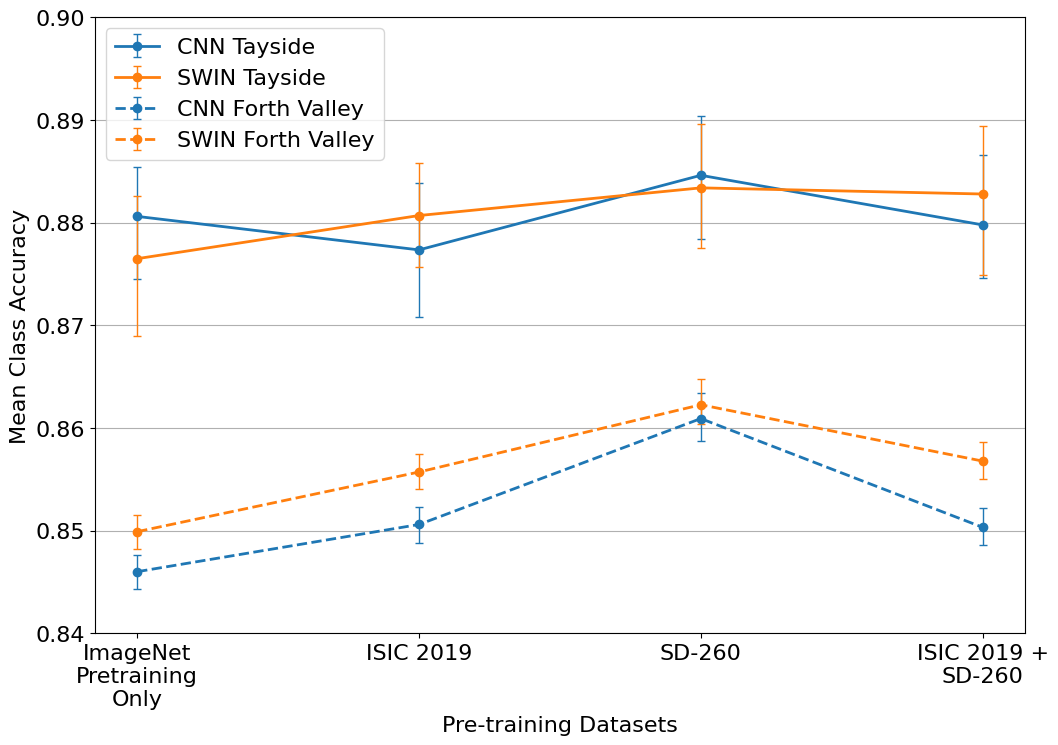
\includegraphics[width=\textwidth]{images/tayside_testing.png}} \\
		\subcaptionbox{\centering Testing on the Forth Valley dataset.}{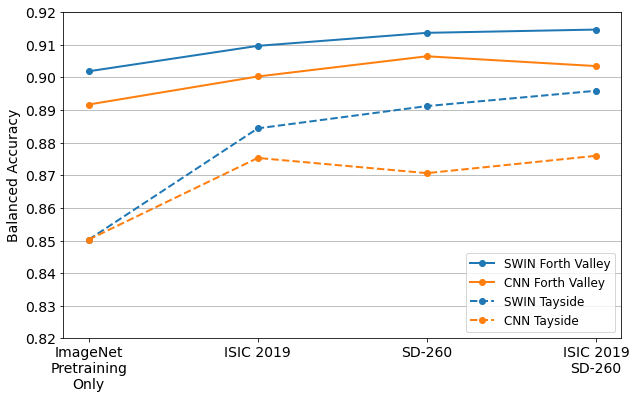
\includegraphics[width=\textwidth]{images/forth_valley_testing.png}}
	\end{tabular}
	\caption{Mean class accuracy results for EfficientNet CNN (blue) and SWIN (orange) benign-malignant classifiers tested on (a) Tayside and (b) Forth Valley data. Bars indicate 95\% tolerance intervals computed using bootstrap. The x-axis indicates the datasets used for pretraining and the image legend indicates the fine-tuning dataset. All classifiers were first pre-trained with ImageNet. Solid lines: fine-tuned on Tayside; Dashed lines: fine-tuned on Forth Valley.}
	\label{fig:generalisation_testing}
\end{figure}

The 95\% confidence intervals shown in Tables \ref{tab:generalisation_results} and \ref{tab:generalisation_models} are always small, always encompassing a range less than $\pm,0.001$. This result indicates a higher level of statistical dependability in the estimated values of the parameters under consideration. It specifically suggests that the models under consideration have a remarkable amount of robustness, and the predictions they provide have a respectable level of resilience. In contrast, the visual representations shown in Figures \ref{fig:generalisation_models}, \ref{fig:generalisation_testing}, and \ref{fig:generalisation_roc} use 95\% tolerance intervals rather than confidence intervals since the latter were regarded too small. These tolerance intervals represent the upper and lower boundaries of the generated bootstrap samples' central 95\% distribution.

Finally, binary classification performance in the form of ROC curves is reported in Figure~\ref{fig:generalisation_roc}. These curves were generated using models pre-trained on SD-260 prior to training on either Tayside or Forth Valley data. It was observed that the Forth Valley curves dominated the Tayside curves, and curves for models trained on the test domain dominated curves trained on the other domain. This occurrence is arguably due to the noticeably higher quality of the Forth Valley photos, as seen in Figure~\ref{fig:nhs_dataset_examples}, primarily in terms of properties such as lighting, spatial alignment, and proportional scale. As a result, the classification model can have a concentrated focus on the knowledge of the key lesion characteristics avoiding involvement with these variables.

\begin{figure}[h]
	\centering
	\captionsetup[subfigure]{singlelinecheck=false}
	\begin{tabular}{c}
		\subcaptionbox{\centering ROC curve for EfficientNet CNN classifiers.}{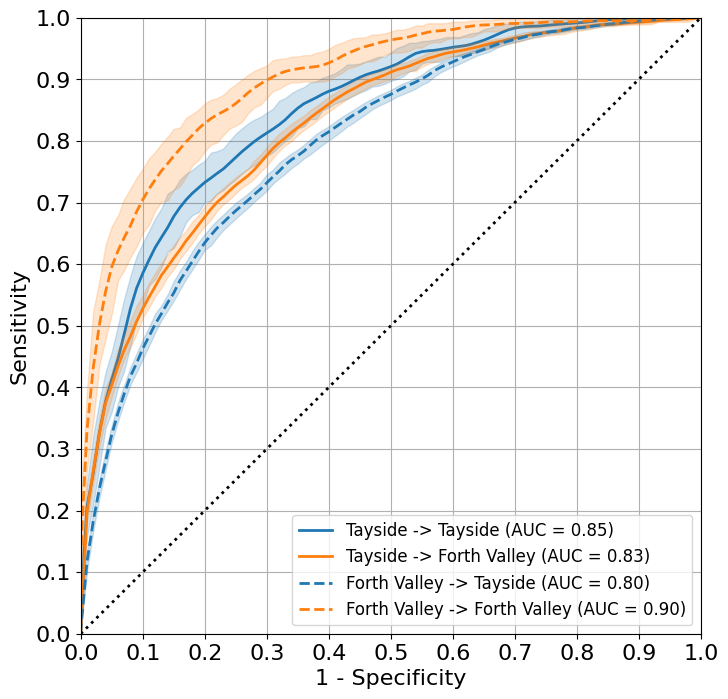
\includegraphics[width=0.8\textwidth]{images/cnn_roc.png}} \\
		\subcaptionbox{\centering ROC curve for SWIN transformer classifiers.}{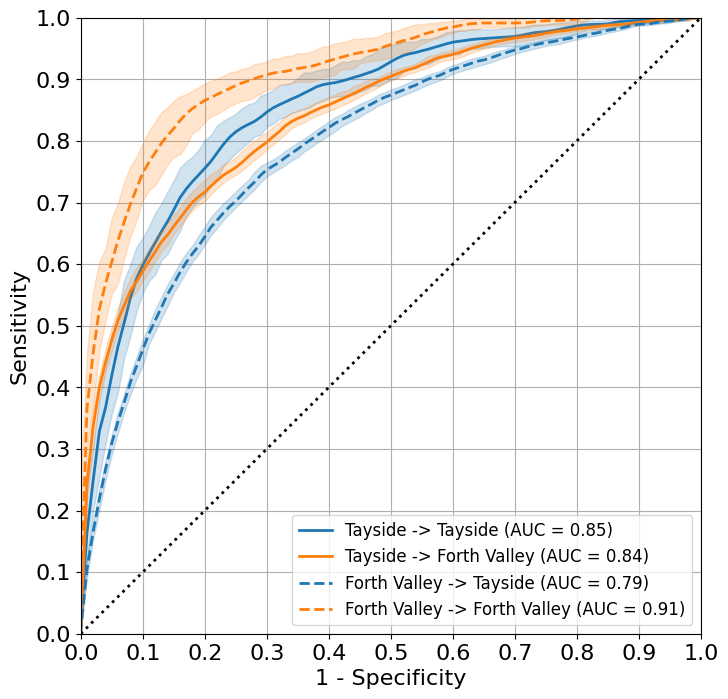
\includegraphics[width=0.8\textwidth]{images/swin_roc.png}}
	\end{tabular}
	\caption{ROC curves for (a) CNN and (b) SWIN classifiers tested on Tayside (blue) and Forth Valley (orange) datasets. All curves were generated using classifiers pre-trained on SD-260 prior to fine-tuning on either Tayside data (solid lines) or Forth Valley data (dashed lines). Shaded areas indicate 95\% tolerance intervals computed using bootstrap.}
	\label{fig:generalisation_roc}
\end{figure}


\section{Conclusion}
\label{sec:generalisation_conclusion}
It is well-established that deep learning classifiers benefit from large training sets. However, it is also known that test performance is negatively affected by variations in image acquisition, image quality, and the population being imaged. This presents challenges in the development of dermatology diagnostic systems that can be deployed in multiple sites, as such conditions can vary geographically and over time. Curation of large datasets can be costly at a local level, yet learning systems need to be attuned to local conditions.

The results suggest that the SWIN transformer should be preferred over the EfficientNet convolutional neural network. The transformer obtained accuracies of 98\% and 97\% on the ISIC 2019 and SD-260 test datasets, provided it was trained on data from the same domain. However, cross-domain fine-tuning (training on ISIC 2019 and testing on SD-260) led to a weaker 79\% accuracy. Training on SD-260 and testing on ISIC 2019 yielded a better 88\% accuracy, possibly due to the more varied nature of the SD-260 dataset (Table~\ref{tab:generalisation_results}).

The ISIC 2019 and SD-260 datasets are relatively large, though still not comparable to datasets used for deep learning in computer vision. The focus of this chapter was how to obtain good performance on challenging local data with limited availability of diagnostic labels. The two NHS datasets used to explore this question were sourced from Tayside and Forth Valley, the latter having images of more consistent and higher quality than the former. Transformers yielded accuracies of 88\% and 90\%, respectively, when trained and tested on data from these domains. This was better than results obtained by training on the larger SD-260 and ISIC 2019 datasets (Figure~\ref{fig:generalisation_models}), highlighting the benefit of training with data from the local target domain. It was found that by pre-training on SD-260 and then on data from the local target domain, further increases to 89\% and 91\% were obtained (Figure~\ref{fig:generalisation_testing}, solid blue lines).

Given their geographical proximity, Tayside and Forth Valley data are from similar populations, so one might expect good cross-domain fine-tuning generalisation between them. However, training on data from one (with appropriate pre-training for transfer) and testing on the other gave accuracies 2-3\% lower than testing on the same domain. This is likely due to differences in image acquisition. ROC curves were used to indicate sensitivity-specificity trade-offs (Figure~\ref{fig:generalisation_roc}). In a triage setting, relatively low specificity can be acceptable in return for very high sensitivity, especially for melanoma. A combination of pre-training on public macroscopic data, followed by tuning to local data, gave promising results. However, further improvements are needed for deployment in a real clinical pathway.